\documentclass[xcolor={usenames,dvipsnames,svgnames}, compress]{beamer}


\usepackage{booktabs}
\usepackage{multirow}
\usepackage{dcolumn}
\usepackage{colortbl}
\usepackage{xcolor}
\usepackage{hyperref}
\usepackage{amsmath}
\usepackage{wrapfig}
\usepackage{algorithm}
\usepackage[noend]{algpseudocode} 
\usepackage{pifont}
\usepackage[style=authoryear-icomp,backend=bibtex, mincitenames=2, maxcitenames=2]{biblatex}
\usepackage{marvosym}
\usepackage{mathtools}
\usepackage{array}
\usepackage[export]{adjustbox}
\usepackage{bm}
\usepackage{dsfont}
\usepackage{subcaption}

\usepackage[font=scriptsize]{caption}


% 
% custom colors
\definecolor{untractable_red}{RGB}{209, 25, 25}
\definecolor{tractable_green}{RGB}{0, 153, 51}

\newcommand{\argmax}{\operatornamewithlimits{argmax}}
\newcommand{\argmin}{\operatornamewithlimits{argmin}}
\newcommand{\nodeset}[1]{\bm{\mathsf{#1}}}
\newcommand{\cbar}{\,|\,}

\newcolumntype{R}[2]{
  >{\adjustbox{angle=#1,lap=\width-(#2)}\bgroup}
  l
  <{\egroup}
}

\newcommand*\rot{\multicolumn{1}{R{45}{1em}}}


%
% Color palette
%
\definecolor{lacamgreen} {RGB} {72, 175, 115}
\definecolor{lacamlilac} {RGB} {107,93,153}
\definecolor{lacamlilac2} {RGB} {93, 109, 152}
\definecolor{lacamlightlilac} {RGB} {174, 166, 201}
\definecolor{lacamdarklilac} {RGB} {51, 10, 102}
\definecolor{lacamgold} {RGB} {255, 87, 0}
\definecolor{lacamdarklilac5} {RGB} {51, 10, 102}
\definecolor{lacamgold5} {RGB} {255, 87, 0}
\definecolor{violet} {RGB} {119, 111, 178}
\definecolor{petroil2} {RGB} {36, 165, 175}
\definecolor{petroil4} {RGB} {30, 132, 149}
\definecolor{petroil6} {RGB} {23, 101, 115}
\definecolor{gold2} {RGB} {255, 130, 0}
\definecolor{gold4} {RGB} {250, 100, 0}
\definecolor{gold6} {RGB} {245, 90, 0}
\definecolor{darkred} {HTML} {67000C}

%\definecolor{tomato0} {HTML} {E57373}
\definecolor{tomato0} {HTML} {EF9A9A}
\definecolor{tomato1} {HTML} {F44336}
\definecolor{tomato2} {HTML} {E53935}
\definecolor{tomato3} {HTML} {D32F2F}
\definecolor{tomato4} {HTML} {C62828}
\definecolor{tomato5} {HTML} {B71C1C}


\definecolor{peas1} {HTML} {009688}
\definecolor{peas2} {HTML} {00897B}
\definecolor{peas3} {HTML} {00796B}
\definecolor{peas4} {HTML} {00695C}
\definecolor{peas5} {HTML} {004D40}

\definecolor{bgrey0} {HTML} {78909C}
\definecolor{bgrey1} {HTML} {607D8B}
\definecolor{bgrey2} {HTML} {546E7A}
\definecolor{bgrey3} {HTML} {455A64}
\definecolor{bgrey4} {HTML} {37474F}
\definecolor{bgrey5} {HTML} {263238}

\definecolor{olive0} {HTML} {C5E1A5}
\definecolor{olive1} {HTML} {AED581}
\definecolor{olive2} {HTML} {9CCC65}
\definecolor{olive3} {HTML} {8BC34A}
\definecolor{olive4} {HTML} {7CB342}
\definecolor{olive5} {HTML} {689F38}

\definecolor{pink0} {HTML} {FCE4EC}
\definecolor{pink1} {HTML} {F8BBD0}
\definecolor{pink2} {HTML} {F48FB1}
\definecolor{pink3} {HTML} {F06292}
\definecolor{pink4} {HTML} {EC407A}
\definecolor{pink5} {HTML} {FF80AB}

\definecolor{brown0} {HTML} {D7CCC8}
\definecolor{brown1} {HTML} {BCAAA4}
\definecolor{brown2} {HTML} {A1887F}
\definecolor{brown3} {HTML} {8D6E63}
\definecolor{brown4} {HTML} {795548}
\definecolor{brown5} {HTML} {6D4C41}
\definecolor{brown6} {HTML} {5D4037}

\definecolor{yellow0} {HTML} {CDDC39}
\definecolor{yellow1} {HTML} {9E9D24}
\definecolor{yellow3} {HTML} {FFBD2A}
\definecolor{yellow4} {HTML} {FFB000}
\definecolor{yellow5} {HTML} {FFD600}



\AtEveryCite{\color{violet}\bf}
% \AtEveryCite{\color{violet}}


\usepackage{calc}

%Define a reference depth. 
%You can choose either relative or absolute.
%--------------------------
\newlength{\DepthReference}
\settodepth{\DepthReference}{g}%relative to a depth of a letter.
%\setlength{\DepthReference}{6pt}%absolute value.

%Define a reference Height. 
%You can choose either relative or absolute.
%--------------------------
\newlength{\HeightReference}
\settoheight{\HeightReference}{T}
%\setlength{\HeightReference}{6pt}


%--------------------------
\newlength{\Width}%

\newcommand{\MyColorBox}[2][red]%
{%
    \settowidth{\Width}{#2}%
    %\setlength{\fboxsep}{0pt}%
    \colorbox{#1}%
    {%      
        \raisebox{-\DepthReference}%
        {%
                \parbox[b][\HeightReference+\DepthReference][c]{\Width}{\centering#2}%
        }%
    }%
}


% \newcommand{\highlight}[2][yellow]{\mathchoice%
%   {\colorbox{#1}{\strut\textcolor{white}{$\displaystyle{#2}$}}}%
%   {\colorbox{#1}{\strut\textcolor{white}{$\textstyle{#2}$}}}%
%   {\colorbox{#1}{\strut\textcolor{white}{$\scriptstyle{#2}$}}}%
%   {\colorbox{#1}{\strut\textcolor{white}{$\scriptscriptstyle{#2}$}}}}%
\newcommand{\highlight}[2][yellow]{\mathchoice%
  {\colorbox{#1}{\textcolor{white}{$\displaystyle{#2}$}}}%
  {\colorbox{#1}{\textcolor{white}{$\textstyle{#2}$}}}%
  {\colorbox{#1}{\textcolor{white}{$\scriptstyle{#2}$}}}%
  {\colorbox{#1}{\textcolor{white}{$\scriptscriptstyle{#2}$}}}}%

%\newcommand{\highlighttext}[2][yellow]{{\colorbox{#1}{\strut\textcolor{white}{#2}}}}
\newcommand{\highlighttext}[2][yellow]{{\colorbox{#1}{\textcolor{white}{#2}}}}
%\newcommand{\highlighttext}[2][yellow]{{\MyColorBox[#1]{\textcolor{white}{#2}}}}



\usetheme{enziteto}

\setbeamertemplate{headline}{}

\newcommand*\samethanks[1][\value{footnote}]{\footnotemark[#1]}

\makeatletter
\renewcommand*{\@fnsymbol}[1]{\ensuremath{\ifcase#1\or $\Yinyang$\or \dagger\or \ddagger\or
    \mathsection\or \mathparagraph\or \|\or **\or \dagger\dagger
    \or \ddagger\ddagger \else\@ctrerr\fi}}
\makeatother

\setbeamerfont{footnote}{size=\scriptsize}
%\addtobeamertemplate{footnote}{}{\vspace{16pt}}
\newcommand{\customcite}[1]{\footnote{\tiny \citeauthor{#1}, \citetitle{#1}, \citeyear{#1}}}
\newcommand{\customcitenomark}[1]{\footnotenomarkleft{\tiny
    \citeauthor{#1}, \citetitle{#1}, \citeyear{#1}}}
\newcommand{\customcitetext}[1]{\footnotenomarkleft{\tiny \citeauthor{#1}, \citetitle{#1}, \citeyear{#1}}}

% 
% custom colors
\definecolor{untractable_red}{RGB}{209, 25, 25}
\definecolor{tractable_green}{RGB}{0, 153, 51}

\newcommand{\cmark}{\ding{51}}%
\newcommand{\xmark}{\ding{55}}

% \bibliographystyle{splncs03}
% \bibliography{../tiselac}

% \newlength{\custombulletheight}
% \setlength{\custombulletheight}{\dimexpr0.5\ht1-0.5\ht2}

\newcommand{\plusbullet}{\raisebox{\custombulletheight}{\hbox{\tiny\textcolor{lacamlilac}{$\boldsymbol{\oplus}$}}\hspace{-2pt}}}

\setbeamertemplate{itemize item}{\raisebox{.21ex}{\hbox{\tiny\textcolor{lacamlilac}{$\boldsymbol{\oplus}$}}\hspace{-2pt}}}
\setbeamertemplate{itemize subitem}{\raise .2ex\hbox{\tiny\textcolor{lacamlilac}{$\boldsymbol{\otimes}$}}\hspace{-3pt}}
\setbeamertemplate{itemize subsubitem}{\textcolor{lacamlilac}{$\oplus$}}
\setbeamertemplate{bibliography item}{\hspace{10pt}\raise .2ex\hbox{\t, 10ptiny\textcolor{lacamlilac}{$\boldsymbol{\oplus}$}}}





\setbeamertemplate{bibliography item}{\hspace{10pt}\raise
  .2ex\hbox{\textcolor{lacamlilac}{$\boldsymbol{\oplus}$}}}

\addbibresource{../referomnia/referomnia.bib}

\begin{document}

\newlength{\custombulletheight}
\setlength{\custombulletheight}{\dimexpr0.5\ht1-0.5\ht2}

\title{{\color{lacamlilac}Encoding and Decoding\\Representations\\with
    Sum-Product Networks}}
\author{\vspace{-10pt}\emph{\textbf{Antonio
      Vergari}}\\\vspace{10pt}joint  work with:\\ Robert
  Peharz, Nicola Di Mauro, Alejandro Molina, Kristian Kersting and Floriana Esposito\\\vspace{10pt}
\includegraphics[width=20pt]{figures/logo1}}
% \institute{Department of Computer Science, University of Bari ``Aldo Moro'', Bari, Italy
% \and 
% Department of Physics, University of Bari ``Aldo Moro'', Bari, Italy
% \and
% National Institute for Nuclear Physics (INFN), Bari Division, Bari, Italy
% }
\institute{University of Bari}
\department{Department of Computer Science}
\laboratory{LACAM Laboratory}
\group{Machine Learning}
 \institutelogo{
\includegraphics[width=25pt]{figures/unibaba}}
%       \hspace{20pt}
%       % \vspace{5pt}
%       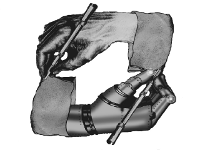
\includegraphics[width=32pt]{figures/lacam}
%       \hspace{20pt}
%       \includegraphics[width=32pt]{figures/fisicalogo}
%       \hspace{25pt}
%       \includegraphics[width=22pt]{figures/infn}}
\lablogo{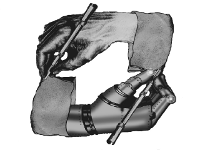
\includegraphics[width=35pt]{figures/lacam}}
\date{November 14th - Bari - AIxIA 2017}

% \makeatletter
% \defbeamertemplate*{title page}{custom-enziteto}[1][]
% {
%   \begin{minipage}[t]{0.9\linewidth}
%     \vspace{0pt}
%     % 
\includegraphics[width=25pt]{Figures/unibaba}
%     \ifdefined\@institutelogo
%     \@institutelogo
%     \fi
%   \end{minipage}
%   \begin{minipage}[t]{0.9\linewidth}
%     \vspace{2pt}
%     \flushleft
%     {\usebeamerfont{institute}\insertinstitute\par}
%     \vspace{2pt}
%     \ifdefined\@department
%     \tiny\@department
%     \fi
%   \end{minipage}
%   \ifdefined\@laboratory
%   %\hspace{10pt}
%   \begin{minipage}[t]{0.12\linewidth}
%     \vspace{0pt}
%     \ifdefined\@lablogo
%     \@lablogo
%     \else
%     \hspace{10pt}
%     \fi
%   \end{minipage}
%   \begin{minipage}[t]{0.40\linewidth}
%     \vspace{7pt}
%     \flushleft
%     \tiny\textbf{\@laboratory}\par
%     \vspace{2pt}
%     \ifdefined\@group
%     \@group
%     \fi
%   \end{minipage}
%   \par
%   \fi
%   \vspace{15pt}
  
%   \Large\usebeamerfont{title}\textcolor{lacamdarklilac5}{\inserttitle}\par%\textcolor{lacamlilac}{\inserttitle}\par
%   \vspace{5pt}
%   \small\usebeamerfont{subtitle}\textcolor{lacamlilac}{\insertsubtitle}\par
%   \vspace{15pt}
%   \usebeamerfont{author}\insertauthor\par
  
%   \ifdefined\@gliph
%   \vspace{7pt}
%   \@gliph\par
%   \vspace{7pt}
%   \else
%   \vspace{21pt}
%   \fi
%   \usebeamerfont{date}\insertdate\par
  
% }
% \makeatother


{
  \setbeamertemplate{headline}{}
  \setbeamertemplate{footline}{}
  \begin{frame}
    \titlepage
  \end{frame}
}

\begin{frame}[t]
  \frametitle{Outline}
  \footnotesize

  Extending \emph{\textbf{Sum-Product Networks}}
  (\textbf{SPNs})~\emph{\parencite{Poon2011}} towards \emph{\textbf{Representation
  Learning}} (\textbf{RL}) by equipping them with encoding and decoding
  routines.
  Learn a density estimator once and exploit it for predictive tasks
  later---without retraining---e.g. \emph{\textbf{Multi-Label Classification}} (\textbf{MLC}).\par\bigskip


  Dealing with categorical---\emph{\textbf{$\mathsf{CAT}$ embeddings}}---and
  continuous  representations---\emph{\textbf{$\mathsf{ACT}$
      embeddings}}---by leveraging the \emph{\textbf{probabilistic latent variable semantics}}
   and the \emph{\textbf{neural network interpretation}} of SPNs, respectively.\par\bigskip


  \highlighttext[tomato2]{\textbf{Density estimation} >}\par
  \hspace{20pt} \highlighttext[tomato3]{\textbf{Sum-Product Networks} >}\par
  \hspace{40pt} \highlighttext[tomato5]{\textbf{MPE inference with SPNs} >}\par
  \hspace{60pt} \highlighttext[bgrey0]{\textbf{CAT embeddings} >}\par
  \hspace{80pt} \highlighttext[bgrey1]{\textbf{ACT embeddings} >}\par
  \hspace{100pt} \highlighttext[bgrey2]{\textbf{CAT vs ACT embeddings} >} \par
  \hspace{120pt} \highlighttext[peas1]{\textbf{MLC predictions} >}\par
  \par\bigskip

  
\end{frame}


\begin{frame}[t]
  \frametitle{\highlighttext[tomato4]{Learn \emph{once}, exploit \emph{more than once}}}
  \footnotesize
  
   The challenges in the arms race to \emph{\textbf{deeply
       make sense of data}}
   lie into the  ability to effectively make use of \highlighttext[tomato0]{\emph{\textbf{unlabeled data}}}
   and to efficiently reason about it, i.e. to make
   \emph{\textbf{inference}} about their configurations and
   relationships\par
   \hfill\begin{minipage}{1.0\linewidth}
    \vspace{5pt}
    \raggedleft
    $\color{violet}\boldsymbol\Rightarrow$
    \scriptsize
    \it
    how to understand the flow of traffic in a city from historical
    records,\par
    traffic light sensors and camera recordings?
    % how to understand\par why congestions happen and how to predict the next ones?
  \end{minipage}\par\bigskip
   % Even the winners of the data arms race cannot make sense of all of
   % it by just building predictive models on them
   %    The arms race to deeply understand data''

   \emph{\textbf{Density estimation}} is the unsupervised task of
    learning an estimator for the joint probability distribution
    $p(\mathbf{X})$ from i.i.d. samples $\mathcal{D}=\{\mathbf
    x^i\}_{i=1}^m$ over random variables (RVs) $\mathbf{X}$
    %$\mathbf{X}=\{X_{1},\dots,X_{n}\}$.
    Given such an estimator, answer a wide range of probabilistic
    queries:\par
    \hfill\begin{minipage}{0.75\linewidth}
    \vspace{5pt}
    \raggedleft
    $\color{violet}\boldsymbol\Rightarrow$
    \scriptsize
    \emph{complete evidence}, \emph{marginals}, \emph{conditionals},\par
    \emph{Most Probable Explanaition} (MPE),\dots % and MAP \emph{assignments},\par
    % \emph{partition function} ($Z$), \emph{sampling} (SAM), \dots
  \end{minipage}\par\bigskip



  %   Given such an estimator, one can \emph{answer
  %   several probabilistic queries} about configurations on $\mathbf{X}$,
  % i.e. to do \emph{\textbf{inference}}.\par

  
    
  % \hfill\begin{minipage}{0.75\linewidth}
  %   \vspace{5pt}
  %   \raggedleft
  %   $\color{violet}\boldsymbol\Rightarrow$
  %   \scriptsize
  %   \emph{complete evidence} (EVA), \emph{marginals} (MAR), \emph{conditionals} (CON),\par
  %   \emph{Most Probable Explanaition} (MPE) and MAP \emph{assignments},\par
  %   \emph{partition function} ($Z$), \emph{sampling} (SAM)
  % \end{minipage}\par\bigskip
  
  % % \begin{itemize}
  % %   \item $p(\mathbf{X} = \mathbf{x})$ pointwise evidence (EVI) 
  % %   \item $p(\mathbf{E}), \mathbf{E}\subset\mathbf{X}$ marginals (MAR)
  % %   \item $p(\mathbf{Q}|\mathbf{E}), \mathbf{Q},
  % %     \mathbf{E}\subset\mathbf{X}, \mathbf{Q}\cap \mathbf{E}=\emptyset$
  % %     conditionals (CON)
  % %   \item $\arg\max_{\mathbf{q}\sim\mathbf{Q}}p(\mathbf{q}|\mathbf{E})$
  % %     MPE assignments (MPE)
  % %   \item $Z =\sum_{\mathbf{x}\sim \mathbf{X}}\phi(\mathbf{x})$
  % %     partition function (Z)
  % %     \item sampling: generate $\mathbf{x}\sim p(\mathbf{X})$ (SAM)
  % %   \end{itemize}


  %   As many machine learning task can be reframed as inference through
  %   $p$ on different configurations on
  %   $\mathbf{X}$,
  %   density estimator qualifies to be \emph{the most general task} to solve.\par
  %   \begin{minipage}{1.0\linewidth}
  %     \vspace{5pt}
  %     \raggedleft
  %     $\color{violet}\boldsymbol\Rightarrow$
  %   \scriptsize\emph{e.g., classification as MPE inference}:
  %   $y^{*}=\argmax_{y\sim Y}p(y|\mathbf{X})$
  %   \end{minipage}\par\bigskip
  

    % The intrinsic trade-off of density estimation: balancing
    % \begin{itemize}
    %   \setlength\itemsep{-3pt}
    % \item the \highlighttext[lacamlilac]{\textbf{\emph{representation
    %         expressiveness}}} of the model to learn
    % \item the \highlighttext[gold4]{\textbf{\emph{cost of learning}}}
    %   such a model
    %   \item and the \highlighttext[petroil2]{\textbf{\emph{cost of performing inference}}} on it
    %   \end{itemize}

  \highlighttext[tomato0]{\textbf{\emph{Learn once, exploit it several times}}} philosophy to
  density estimation: learn one \emph{tractable} probabilistic model
  in an unsupervised way from data, \emph{then}:
  \begin{itemize}
  \item perform (several kinds of) \emph{\textbf{inference ad
        libitum}}
    \item \emph{\textbf{exploit it for predictive tasks}} later, without training again
  \end{itemize}

\end{frame}

%   \begin{frame}[t]
%     \frametitle{\highlighttext[tomato4]{Learn \emph{once}, exploit \emph{more than once}}}
%     \footnotesize
    
%     Learn one SPN $S$ generatively from data
%     $\{\mathbf{x}^{i}\sim\mathbf{X}\}_{i=1}^{m}$ to estimate
%     $p(\mathbf{X})$ and then exploit it into other tasks---\emph{without
%     retraining} it---by interpreting it as a neural network:
%     \begin{itemize}
%     \item as a feature extractor for Representation Learning (RL)\par
%       \begin{minipage}{1.0\linewidth}
%  %     \vspace{2pt}
%       \raggedleft
%       $\color{violet}\boldsymbol\Rightarrow$
%       \scriptsize
%      \emph{sum, product nodes or scope aggregations as filters}
%       \end{minipage}~\customcite{Vergari2016a}
% \item as an auto-encoder mapping back and forth embeddings\par
%   \begin{minipage}{1.0\linewidth}
% %  \vspace{2pt}
%       \raggedleft
%       $\color{violet}\boldsymbol\Rightarrow$
%       \scriptsize
%  \emph{Sum-Product Autoencoding}
% \end{minipage}~\customcite{Vergari2017}
% \item understanding learned representations\par
%   \begin{minipage}{1.0\linewidth}
% %  \vspace{2pt}
%       \raggedleft
%       $\color{violet}\boldsymbol\Rightarrow$
%       \scriptsize
%  \emph{visualizing filters in the input space}
% \end{minipage}% ~\customcite{Vergari2016a}
%     \end{itemize}\par\bigskip
%     % Solving different query types exactly and efficiently (linear to
%     % the network size)\par\bigskip

%     Moreover the interpretation of SPNs as NNs enables
%     \begin{itemize}
%       %\setlength{\itemsep}{-3pt}
%     % \item extracting embeddings as neuron activations
%     \item efficient implementations running on GPUs
%     \item structure learning as a constrained optimization problem
      
%     \end{itemize}


%     % \textbf{\emph{Sum-Product Autoencoding}}
%     % (\textbf{SPAE})\customcite{Vergari2017}, 

%     %  by interpreting SPNs as NNs Extracting embeddings to be used for
%     %  supervised, semi-supervised predictive tasks~\customcite{Vergari2016a}~\customcite{Vergari2016b}:
%     %  \begin{itemize}
%     %  \item filterning nodes: sum, products
%     %  \item identifying hierarchies of abstractions by scopes
%     %  \item aggregating scope information
%     %  \item categorical embedding from latent variable semantics
%     %  \end{itemize}\par\bigskip

%     %  Interpreting them as Autoencoders by providing decoding routines
%     %  for embeddings, leveraging MPE inference~\customcite{Vergari2017}
       
%   \end{frame}
  



  \begin{frame}[t]
    \frametitle{\highlighttext[tomato3]{Sum-Product Networks (SPNs)}}
    \footnotesize
      A \emph{Sum-Product Network} $S$ over RVs $\mathbf X$ is defined via
  rooted weighted DAG consisting of
  distribution \highlighttext[purple]{\emph{\textbf{leaves}}} (network inputs),  \highlighttext[gold2]{\emph{\textbf{sum}}} and \highlighttext[petroil2]{\emph{\textbf{product}}}
  nodes (inner nodes).

  \vspace{0.5 cm}

  Each sub-network $S_{n}$ defines an unnormalized probability
  distribution over the subset of RVs appearing in it, $\mathsf{sc}(n)\subseteq\mathbf X$.\par\bigskip
\begin{minipage}{0.63\textwidth}
\begin{itemize}
\item  A % \emph{\color{purple}\textbf{leaf}}
  leaf
  $n$ defines a \textbf{tractable distribution}\par
  %$\highlight[purple]{\phi_{n}(\mathbf{x})=
  %p(\mathbf{x}_{|\mathsf{sc}(n)})}$
  \hfill ${\color{purple}\phi_{n}(\mathbf{x})}= p(\mathbf{x}_{|\mathsf{sc}(n)})$
  % over $\mathsf{scope}(n)\subseteq\mathbf X$.
\item a % \emph{\color{petroil2}\textbf{product node}}
  product node
      $n$ represents a \textbf{factorization over independent
        components}\par
      %$\highlight[petroil2]{S_{n}(\mathbf{x})=\prod_{c\in
      %\mathsf{ch}(n)}S_{c}(\mathbf{x})}$
      \hfill${\color{petroil2}S_{n}(\mathbf{x})}=\prod_{c\in \mathsf{ch}(n)}S_{c}(\mathbf{x})$

  
\item a % \emph{\color{gold2}\textbf{sum node}}
  sum node
    $n$  denote a
    \textbf{mixture} over its children distributions% , summing out a
    % \emph{\textbf{latent RV}} (\textbf{LV})
    \par
    %$\highlight[gold2]{S_{n}(\mathbf{x})=\sum_{c\in
    %\mathsf{ch}(n)}w_{nc}S_{c}(\mathbf{x})}$
    \hfill ${\color{gold2}S_{n}(\mathbf{x})}=\sum_{c\in \mathsf{ch}(n)}w_{nc}S_{c}(\mathbf{x})$
% where  a nonnegative weight $w_{nc}$ is associated to each edge linking a sum node
%   $n$ to $c\in\mathsf{ch}(n)$
% \begin{itemize}
% \item $\mathsf{ch}(n)$:  child (input) nodes of   a node $n$ 
% \item $\mathsf{pa}(n)$:  parent (output) nodes of a node $n$
% \item $S_{n}$: sub-network rooted at node $n$ 
% \end{itemize}
\end{itemize}


\end{minipage}\hspace{15pt}
\begin{minipage}{0.28\textwidth}
  \vspace{-20pt}
\centering
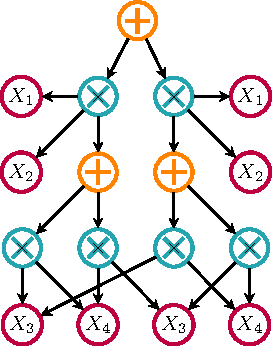
\includegraphics[width=0.85\columnwidth]{figures/spn-colored}
\end{minipage}

  \end{frame}



\begin{frame}[t]
  \frametitle{\highlighttext[tomato3]{Inference with SPNs}}
  \footnotesize
  An SPN $S$ over $\mathbf{X}$  allows the \textbf{\emph{exact}} computation of \emph{{complete evidence}},
  \emph{{marginal}} and {\emph{conditional}} queries for
  $p(\mathbf{X})$ in \emph{\textbf{time linear}} in the network size
  (\# edges, e.g. $|S|$).\par\bigskip
   Exact \emph{\textbf{MPE inference}}, however, is NP-hard in general
 SPNs~\customcite{Peharz2016} but can be answered in exactly in linear
 time in \emph{\textbf{selective SPNs}} % ~\customcite{Peharz2014b}
 by the $\mathsf{MaxProdMPE}$ algorithm.% ~\customcite{Chan2006}
 %\vspace{-10pt}

  \begin{figure}[!ht]
    % \centering
    \raggedright
     \begin{subfigure}[b]{0.15\columnwidth}
     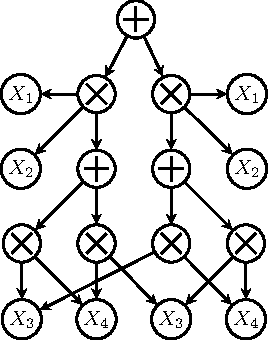
\includegraphics[width=1.0\columnwidth]
     {figures/mpn-eval-i}  
   \end{subfigure}\hspace{5pt}\parbox[b][30pt][b]{0.03\columnwidth}{\subcaption{\label{fig:mpn-eval-i}}}\hspace{15pt}
   \begin{subfigure}[b]{0.15\columnwidth}
     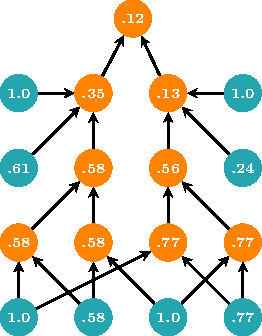
\includegraphics[width=1.0\columnwidth]
     {figures/mpn-eval-ii}% \caption{\label{fig:mpn-eval-ii}}
   \end{subfigure}\hspace{5pt}\parbox[b][30pt][b]{0.03\columnwidth}{\subcaption{\label{fig:mpn-eval-ii}}}\hspace{15pt}
   \begin{subfigure}[b]{0.15\columnwidth}
     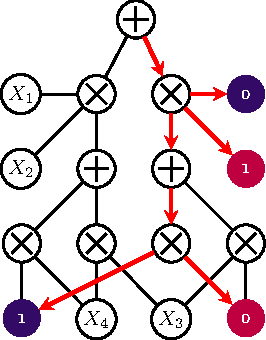
\includegraphics[width=1.0\columnwidth]
     {figures/mpn-eval-iii}% \caption{\label{fig:mpn-eval-iii}}
   \end{subfigure}\hspace{5pt}\parbox[b][30pt][b]{0.03\columnwidth}{\subcaption{\label{fig:mpn-eval-iii}}}
 \end{figure}%\customcitenomark{Vergari2017}


$\mathsf{MaxProdMPE}$ turns $S$ into a \emph{\textbf{Max-Product
     Network}} (\textbf{MPN}) $M$ \emph{(a)}, then evaluates $M$ \textbf{bottom-up}
 propagating evidence and marginalizing over query RVs \emph{(b)}.
A Viterbi-style step
retrieves the query RV assignments \highlighttext[tomato0]{\emph{\textbf{growing a tree
path}} \textbf{top-down}} ---following max sum node child branches and all
product node children \emph{(c)}.

 % % Propagating node activations bottom-up when turned into an MPN to solve
 % %     $\argmax\nolimits_{\mathbf{q}\sim\mathbf{Q}}S(\mathbf{q},X_{2}=1,X_{4}=0)$,
 % %     %its bottom-up evaluation when turned into an MPN to solve $\argmax\nolimits_{\mathbf{q}\sim\mathbf{Q}}p(\mathbf{q},X_{2}=1,X_{4}=0)$,
 % %      $\mathbf{Q}=\{X_{1},X_{3}\}$ (b).
 %     Marginalized nodes in blue activations.
 %     The tree $\theta$ (red) induced  by $\mathsf{MaxProdMPE}$ in the top-down
 %     traversal of $M$ (c).
 %     The assignment for RVs $\mathbf{Q}$ (resp. $\mathbf{O}=\{X_{2},X_{4}\}$) labels the violet
 %     (resp. purple) leaves.
\end{frame}



\begin{frame}[t]
  \frametitle{\highlighttext[bgrey0]{Sum-Product Autoencoding (SPAE)}}
  \footnotesize

  % Extending an SPN $S$---\emph{\textbf{unsupervisedly learned}} to
  % estimate $p(\mathbf{X})$---towards Representation Learning by
  % equipping it with a pair of transformations $f$ and $g$.\par\bigskip

  Given an SPN $S$---\emph{\textbf{unsupervisedly learned}} to
  estimate $p(\mathbf{X})$ we want to {\textbf{\emph{encode}}} a sample
  $\mathbf{x}^{i}\sim\mathbf{X}$ as an \emph{embedding} $\mathbf{e}^{i}$ in a new $d$-dimensional
space $\mathbf{E}_{\mathbf{X}}\subseteq\mathbb{R}^{d}$
    % into $\mathbf{e}^{i}\in\mathbf{E}_{\mathbf{X}}, \mathbf{e}^{i} =
    % f_{S}(\mathbf{x}^{i})$ then decode it back as $g_{S}(\mathbf{e}^{i}) =
    % {\tilde{\mathbf{x}}}^{i}\approx{{\mathbf{x}}}^{i}$.
    $$\mathbf{e}^{i} = f_{S}(\mathbf{x}^{i}).$$

 For \textbf{\emph{decoding}}, on the other hand, we seek an inverse function
$g\colon\mathbf{E}_{\mathbf{X}}\rightarrow\mathbf{X}$ such that
$$ g_{S}(\mathbf{e}^{i}) =
{\tilde{\mathbf{x}}}^{i}\approx{{\mathbf{x}}}^{i}.$$
%is its reconstruction in the original feature space $\mathbf{X}$.\par\bigskip

% The embedding $\mathbf{e}^{i}$ 
% can be the result of an encoding
% process $f_{S}$ \emph{or} the output of a predictive model whose target space
% is $\mathbf{E}_{\mathbf{X}}$.
Embeddings over $\mathbf{X}$ can be later used in {\textbf{\emph{predictive
  tasks}}} as features:
\begin{minipage}{1.0\linewidth}
 %     \vspace{2pt}
      \raggedleft
      $\color{violet}\boldsymbol\Rightarrow$
      \scriptsize
     \emph{e.g. \highlighttext[tomato0]{\emph{\textbf{to predict}}} a RV $Y$% :
       % {\scriptsize${(\mathbf{X}\xrightarrow{\scriptscriptstyle f_{S}}\mathbf{E}_{\mathbf{X}})\xRightarrow{\scriptscriptstyle \mathsf{LR}}\mathbf{Y}}$}
     }
\end{minipage}\\[5pt]
or as the output of a predictive model $p$ whose target space
is $\mathbf{E}_{\mathbf{X}}$
\begin{minipage}{1.0\linewidth}
 %     \vspace{2pt}
      \raggedleft
      $\color{violet}\boldsymbol\Rightarrow$
      \scriptsize
     \emph{e.g. \highlighttext[tomato0]{\emph{\textbf{to disentangle}}} label dependencies $\mathbf{Y}$ in MLC% : {\scriptsize${\quad(\mathbf{X}\xRightarrow{\scriptscriptstyle
             % p}(\mathbf{Y}\xrightarrow{\scriptscriptstyle
             % f_{S}}\mathbf{E}_{\mathbf{Y}}))\xrightarrow{\scriptscriptstyle
             % g_{S}}\mathbf{Y}}$}
     }
\end{minipage}\par\bigskip

We equip $S$ with $f_{S}$ and $g_{S}$ by exploiting MPE inference routines
\begin{minipage}{1.0\linewidth}
  \vspace{5pt}
  \raggedleft
  $\color{violet}\boldsymbol\Rightarrow$
      {\scriptsize
     \emph{dealing with categorical and continuous representations}}\par
      $\color{violet}\boldsymbol\Rightarrow$
      {\scriptsize
     \emph{dealing with \highlighttext[tomato0]{\emph{\textbf{partial embeddings}}}}}
   \end{minipage}\par\bigskip




  %  \begin{figure}[!ht]
 %   \centering
 %   % width: width=0.20\columnwidth
 %   % hspace: 25pt
 %   \setlength{\tabcolsep}{3pt}
 %    \begin{tabular}{ccccc}
 %     \includegraphics[width=0.17\columnwidth]
 %     {figures/spn-mpe-aug-eval-i} \label{fig:spn-aug-eval-i}&
 %     \includegraphics[width=0.17\columnwidth]
 %     {figures/spn-mpe-aug-eval-ii} \label{fig:spn-aug-eval-ii}&
 %     \includegraphics[width=0.17\columnwidth]
 %     {figures/spn-mpe-aug-eval-iii} \label{fig:spn-aug-eval-iii}&
 %     \includegraphics[width=0.17\columnwidth]
 %     {figures/spn-mpe-aug-eval-iiii} \label{fig:spn-aug-eval-iiii}&
 %     \includegraphics[width=0.17\columnwidth]
 %     {figures/spn-mpe-aug-eval-v} \label{fig:spn-aug-eval-v}
 %     %(a) & (b) & (c) & (d) & (e)
 %    \end{tabular}
 % \end{figure}\customcitenomark{Vergari2017}

%  Encoding and decoding $\mathsf{CAT}$egorical embeddings via SPN LV interpretation:
%  \begin{align*}
% f_{S}(\mathbf{x}^{i}) 
%   &= f_{\mathsf{CAT}}(\mathbf{x}^{i}) \triangleq \tilde{\mathbf{z}}^{i}
%   = \argmax\nolimits_{\mathbf{z}^i}S(\mathbf{z}^i \cbar
%   \mathbf{x}^{i})\\
%   g_{S}(\tilde{\mathbf{z}}^{i}) 
%   &= g_{\mathsf{CAT}}(\tilde{\mathbf{z}}^{i}) \triangleq \tilde{\mathbf{x}}^{i} = \argmax\nolimits_{\mathbf{x}^i} S(\mathbf{x}^i \cbar \tilde{\mathbf{z}}^{i})
%  \end{align*}\par\bigskip


% Encoding continuous embedding via node $\mathsf{ACT}$ivations as for
% classical NNs. Decoding by mimicking MPE inference
\end{frame}

   

\begin{frame}[t]
    \frametitle{\highlighttext[bgrey1]{$\mathsf{CAT}$ embeddings (I)}}
    \footnotesize

    Given an SPN $S$ over $\mathbf{X}$,  to each sum node
    $n\in\nodeset{S}^{\oplus}$ is associated a \emph{\textbf{categorical latent
    variable}} (\textbf{LV}) $Z_{n}$
    having values $z_{n}\in\{0,\dots,|\mathsf{ch}(n)|-1\}$.\par\bigskip

    It would be natural to encode $\mathbf{x}^{i}$ through
    the  LVs in $S$,
    i.e. $\mathbf{E}_{\mathbf{X}}=\mathbf{Z}_{S}$ ($d=|\nodeset{S}^{\oplus}|$):
%via MPE inference:
%
% encoding
\begin{equation}
  \label{eq:lv-enc}
  f_{S}(\mathbf{x}^{i}) 
  = f_{\mathsf{CAT}}(\mathbf{x}^{i}) \triangleq \tilde{\mathbf{z}}^{i} = \argmax\nolimits_{\mathbf{z}^i}p(\mathbf{z}^i \cbar \mathbf{x}^{i}),
\end{equation}
% with $\tilde{\mathbf{z}}^{i}$ being the \emph{categorical} vector
% comprising the most probable state for the LVs in $S$, $\tilde{z}_{j}^{i}\sim Z_{j}$.
i.e. $\mathbf{x}^{i}$ is encoded as the \emph{categorical} vector
$\tilde{\mathbf{z}}^{i}$ %---also explaining the name of the embeddings: {\bf CAT}egorial---
comprising the \highlighttext[tomato0]{\emph{\textbf{MPE state}}} for $\mathbf{Z}_{S}$.\par\bigskip
% ($\mathsf{CAT}$ embedding).
%
% decoding
Analogously, the decoding of $\tilde{\mathbf{z}}^{i}$
 through $g_{S}$ can be defined as:
% Analogously, given an encoded sample $\tilde{\mathbf{z}}^{i}$,
% its decoding through $g_{S}$ can be defined as:
\begin{equation}
  \label{eq:lv-dec}
  g_{S}(\tilde{\mathbf{z}}^{i}) 
  = g_{\mathsf{CAT}}(\tilde{\mathbf{z}}^{i}) \triangleq \tilde{\mathbf{x}}^{i} = \argmax\nolimits_{\mathbf{x}^i} p(\mathbf{x}^i \cbar \tilde{\mathbf{z}}^{i}).
\end{equation}\\[10pt]

However, this requires performing MPE inference over the \highlighttext[tomato0]{\emph{\textbf{joint
probability distribution}}} over $\mathbf{V}=(\mathbf{X}, \mathbf{Z}_{S})$

\begin{minipage}{1.0\linewidth}
 %     \vspace{2pt}
      \raggedleft
      $\color{violet}\boldsymbol\Rightarrow$
      \scriptsize
     \emph{we need to deal with an \emph{\textbf{augmented
           SPN}}~\customcite{Peharz2016} $\overline{S}$ over $\mathbf{V}$}
\end{minipage}
    
 %     \begin{figure}[!ht]
 %   \centering
 %   % width: width=0.20\columnwidth
 %   % hspace: 25pt
 %   \setlength{\tabcolsep}{3pt}
 %    \begin{tabular}{ccccc}
 %     \includegraphics[width=0.17\columnwidth]
 %     {figures/spn-mpe-aug-eval-i} \label{fig:spn-aug-eval-i}&
 %     \includegraphics[width=0.17\columnwidth]
 %     {figures/spn-mpe-aug-eval-ii} \label{fig:spn-aug-eval-ii}&
 %     \includegraphics[width=0.17\columnwidth]
 %     {figures/spn-mpe-aug-eval-iii} \label{fig:spn-aug-eval-iii}&
 %     \includegraphics[width=0.17\columnwidth]
 %     {figures/spn-mpe-aug-eval-iiii} \label{fig:spn-aug-eval-iiii}&
 %     \includegraphics[width=0.17\columnwidth]
 %     {figures/spn-mpe-aug-eval-v} \label{fig:spn-aug-eval-v}
 %     %(a) & (b) & (c) & (d) & (e)
 %    \end{tabular}
 % \end{figure}\customcitenomark{Vergari2017}



% Encoding continuous embedding via node $\mathsf{ACT}$ivations as for
% classical NNs. Decoding by mimicking MPE inference
\end{frame}

\begin{frame}[t]
    \frametitle{\highlighttext[bgrey1]{$\mathsf{CAT}$ embeddings (II)}}
    \footnotesize

    \begin{figure}[!ht]
      \vspace{-10pt}
  \raggedright
   %\centering
   % width: width=0.20\columnwidth
   % hspace: 25pt
   \setlength{\tabcolsep}{3pt}
    \begin{tabular}{ccccc}
     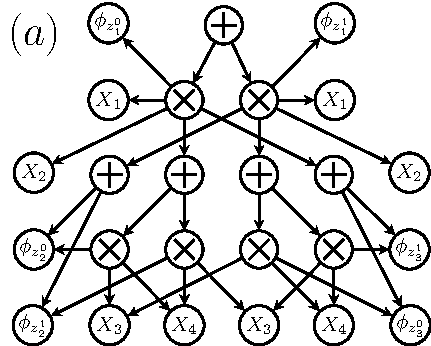
\includegraphics[width=0.17\columnwidth]
     {figures/spn-mpe-aug-eval-i} \label{fig:spn-aug-eval-i}&
     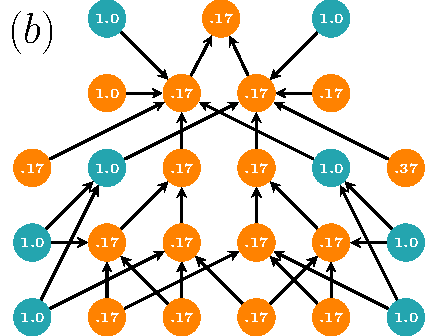
\includegraphics[width=0.17\columnwidth]
     {figures/spn-mpe-aug-eval-ii} \label{fig:spn-aug-eval-ii}&
     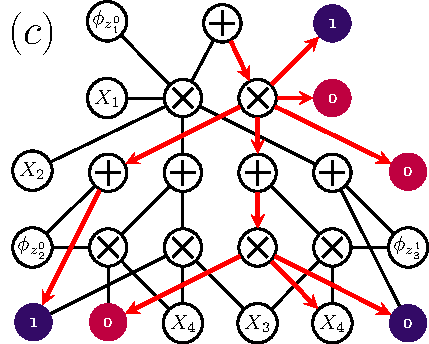
\includegraphics[width=0.17\columnwidth]
     {figures/spn-mpe-aug-eval-iii} \label{fig:spn-aug-eval-iii}&
     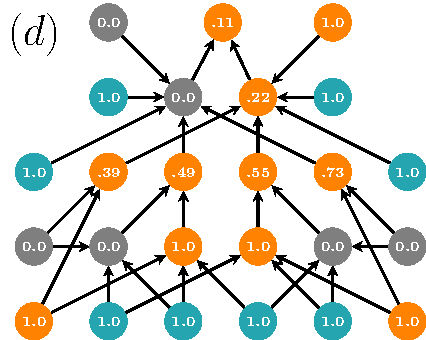
\includegraphics[width=0.17\columnwidth]
     {figures/spn-mpe-aug-eval-iiii} \label{fig:spn-aug-eval-iiii}&
     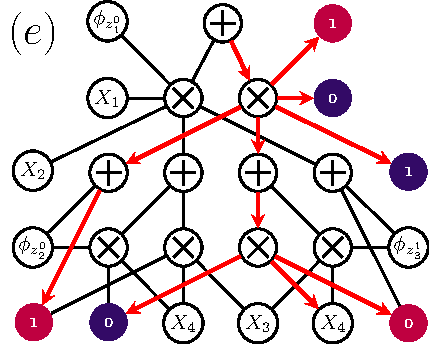
\includegraphics[width=0.17\columnwidth]
     {figures/spn-mpe-aug-eval-v} \label{fig:spn-aug-eval-v}
     %(a) & (b) & (c) & (d) & (e)
    \end{tabular}
 \end{figure}

    % Augmented SPNs allow to employ the same SPN inference machinery
    % over $\mathbf{V}$.\par
    To solve both Eq.~\eqref{eq:lv-enc} and Eq.~\eqref{eq:lv-dec}, 
has to be run
$\mathsf{MaxProdMPE}$ twice on the augmented MPN $\overline{M}$.
Since each application of $\mathsf{MaxProdMPE}$ involves a bottom-up and a backtracking pass, we need in total 4 passes over $\overline{M}$.
\begin{minipage}{1.0\linewidth}
 %     \vspace{2pt}
      \raggedleft
      $\color{violet}\boldsymbol\Rightarrow$
      \scriptsize
     \emph{$\overline{M}$ is selective, hence MPE inference is exact!}
\end{minipage}\par\bigskip
    

Materializing $\overline{M}$ scales quadratically, thus we directly use $M$, evaluating $M(\mathbf{x}^{i})$ in a bottom-up
pass once and then \highlighttext[tomato0]{\emph{\textbf{growing a tree path}}} $\theta$ while collecting the states:
\begin{equation}
  \label{eq:cat-appr}
  z_{j}^{i} = \argmax\nolimits_{k\in\{0, \dots, |\mathsf{ch}(n_j)|\}}w_{n_{j}c_{k}}M_{c_{k}}(\mathbf{x}^{i}),
\end{equation}
for each $Z_{j}\in\mathbf{Z}^{{\theta}}_{S}$, where
$\mathbf{Z}^{{\theta}}_{S}$ are the LVs associated only to the max nodes in
$\theta$.
\begin{minipage}{1.0\linewidth}
 %     \vspace{2pt}
      \raggedleft
      $\color{violet}\boldsymbol\Rightarrow$
      \scriptsize
     \emph{$\mathsf{CAT}$ embeddings are very \highlighttext[tomato0]{\emph{\textbf{sparse}}}!}
\end{minipage}
    


% Encoding continuous embedding via node $\mathsf{ACT}$ivations as for
% classical NNs. Decoding by mimicking MPE inference
\end{frame}

\begin{frame}[t]
  \frametitle{\highlighttext[bgrey1]{$\mathsf{CAT}$ embeddings (III)}}
  \footnotesize
  $\mathsf{CAT}$ embeddings are \highlighttext[tomato0]{\textbf{\emph{compact} and \emph{linear}
  representations of trees \emph{{}}}}, the \textbf{induced trees} in $S$~\customcite{Zhao2015}.\par\bigskip

  % 
We can interpret the semantics of $\mathsf{CAT}$ embeddings
by visualizing \highlighttext[tomato0]{\emph{\textbf{the latent factors of variations}}} encoded in $\mathbf{Z}_{S}$ 
through the \emph{clusters} of samples sharing the same
representations~\customcite{Vergari2016a}.

\begin{figure}[!t]
  % \centering
  \raggedright
  %\subfloat[]{
    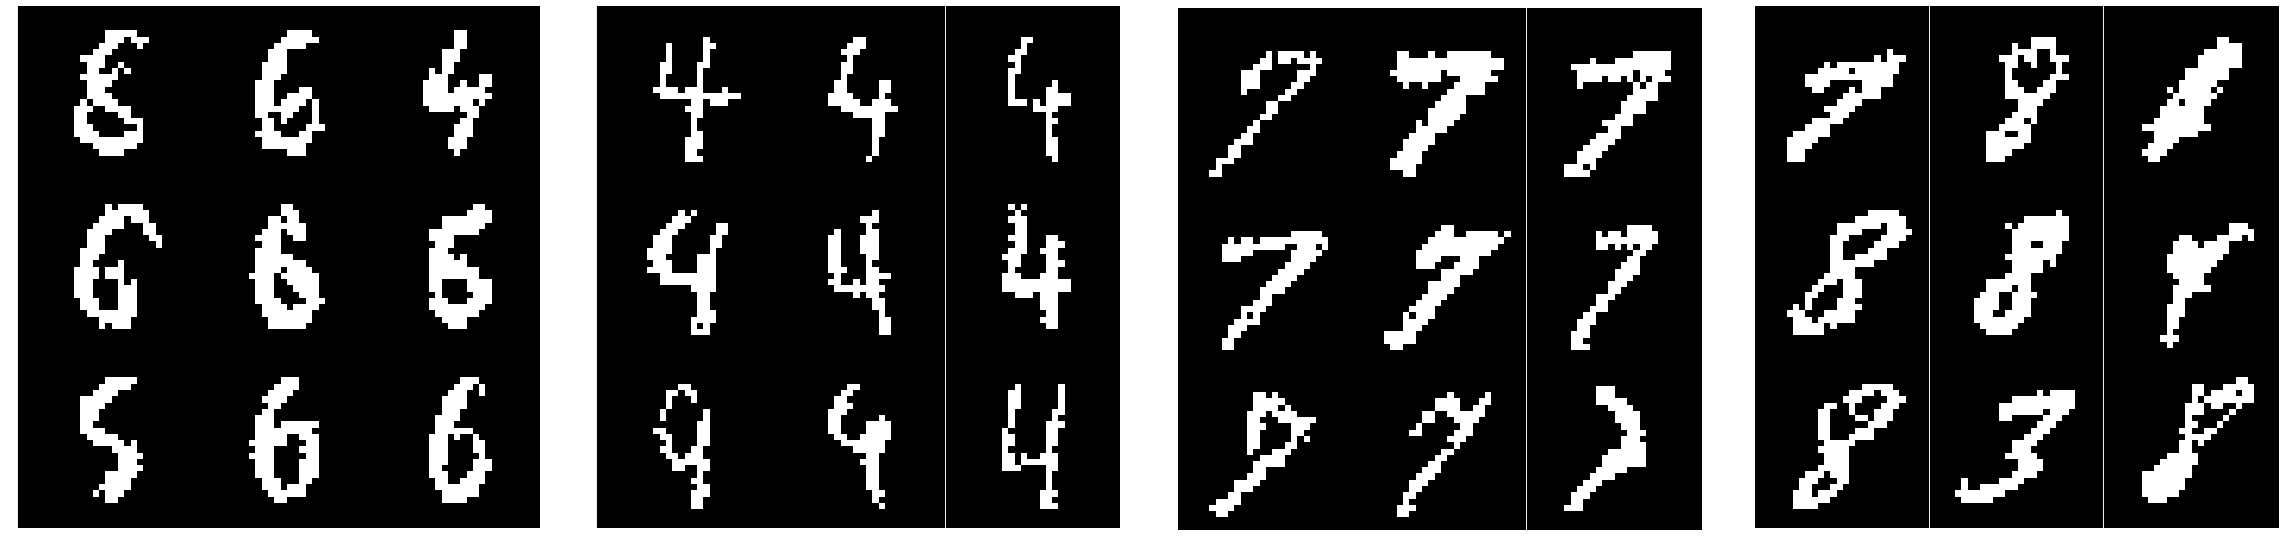
\includegraphics[width=0.75\columnwidth]
    {figures/hid-clu} \label{fig:hid-clu}%}\hspace{6pt}
  \label{fig:bmnist-hid}
\end{figure}
%
%
\vspace{-5pt}
For an SPN learned on MNIST, samples sharing the
same $\mathsf{CAT}$ encoding---even if belonging to different classes, 
clearly 
share \emph{\textbf{stylistic aspects}} like \emph{orientation} and \emph{stroke}.

\end{frame}

\begin{frame}[t]
  \frametitle{\highlighttext[bgrey2]{$\mathsf{ACT}$ embeddings (I)}}
  \footnotesize
SPNs  be interpreted as deep neural networks
with sparse \textbf{\emph{constrained topology}} in which neurons \highlighttext[tomato0]{{\textbf{\emph{labeled}}}} by the scope function $\mathsf{sc}$---enabling a \emph{direct encoding} of the input% ~\cite{Bengio2012}
---retaining a \highlighttext[tomato0]{\emph{\textbf{fully probabilistic
semantics}}}~\customcite{Vergari2016a}.
\begin{minipage}{1.0\linewidth}
 %     \vspace{2pt}
      \raggedleft
      $\color{violet}\boldsymbol\Rightarrow$
      \scriptsize
     \emph{each neuron activation, i.e. $S_{n}(\mathbf{x})$, is a valid probability}
\end{minipage}\par\bigskip

Therefore, neuron \emph{\textbf{$\mathsf{ACT}$ivations}} can be used
as features to build embeddings, 
as it is common practice for neural networks and
autoencoders~\parencite{Rifai2011,Marlin2010}
\begin{minipage}{1.0\linewidth}
 %     \vspace{2pt}
      \raggedleft
      $\color{violet}\boldsymbol\Rightarrow$
      \scriptsize
     \emph{however \highlighttext[tomato0]{\emph{\textbf{representations are not arranged layer-wise}}}!}
\end{minipage}\par\bigskip

Let $\nodeset{N}=\{n_{j}\}_{j=1}^{d}\subseteq\nodeset{M}$
 be a set of nodes
in an MPN $M$, by a \emph{certain criterion}.
A sample $\mathbf{x}^{i}$ is encoded into a $d$-dimensional
\textbf{\emph{continuous}} embedding
$f_{S}(\mathbf{x}^{i}) = \mathbf{e}^{i}\in\mathbf{E}_{\mathbf{X}}\subseteq\mathbb{R}^{d}$
by collecting the activations of nodes in $\nodeset{N}$, i.e.
$$e_{j}^{i}=M_{n_{j}}(\mathbf{x}^{i})$$.

\end{frame}


\begin{frame}[t]
  \frametitle{\highlighttext[bgrey2]{$\mathsf{ACT}$ embeddings (II)}}
  \footnotesize
  We can note how \highlighttext[tomato0]{\textbf{\emph{$\mathsf{ACT}$ embeddings implicitly encode an induced tree}}}: 
node activations $\mathbf{e}^{i}_{M}$ are sufficient to determine
which max node child branch to follow, according to
Eq.~\ref{eq:cat-appr}---recompute each hard decision again.\par\bigskip

Therefore, we can build a decoder $g_{\mathsf{ACT}}$ that \emph{\textbf{mimicks only
the
top-down pass}} of $\mathsf{MaxProdMPE}$: growing the induced tree from
the root by following the max sum node child branches---all product
child nodes are followed as usual.\par\bigskip

Given an SPN $S$ over $\mathbf{X}$---equipped with $(f_{\mathsf{CAT}},
g_{\mathsf{CAT}})$ and $(f_{\mathsf{ACT}}, g_{\mathsf{ACT}})$---and a sample $\mathbf{x}^{i}\sim \mathbf{X}$, 
%   let $\tilde{\mathbf{z}}^{i}$ be its $\mathsf{CAT}$ embedding
%   through
%   $f_{\mathsf{CAT}}$ and $\mathbf{e}^{i}_{M}$ be its
%   $\mathsf{ACT}$ embedding through $f_{\mathsf{ACT}}$.
  it holds
  that:
  \begin{equation}
  g_{\mathsf{ACT}}(f_{\mathsf{ACT}}(\mathbf{x}^{i}))=g_{\mathsf{CAT}}(f_{\mathsf{CAT}}(\mathbf{x}^{i})).\label{eq:cat-act-eq}
\end{equation}
  \begin{minipage}{1.0\linewidth}
     %\vspace{-22pt}
      \raggedleft
      $\color{violet}\boldsymbol\Rightarrow$
      \scriptsize
     \emph{different embeddings, but \highlighttext[tomato0]{\textbf{\emph{equivalent reconstructions}}}!}
   \end{minipage}
\end{frame}


\begin{frame}[t]
  \frametitle{\highlighttext[bgrey2]{$\mathsf{ACT}$ embeddings (III)}}
  \footnotesize
Since $\mathsf{ACT}$ embeddings are points  in
the space induced by a collection of \emph{distributions}, SPN nodes are \highlighttext[tomato0]{\textbf{\emph{part-based filters}}} 
operating over different sub-spaces of RVs.\par\bigskip

For an SPN $S$ we can visualize the filter 
  encoded by sub-network $S_{n}$ rooted at
  node $n$ by \emph{\textbf{computing the
      mode}} of the distribution $p_{S_{n}}$:
  $$\mathbf{x}^{*}_{|\mathsf{sc}(n)} =
  \argmax_{\mathbf{x}}S_{n}(\mathbf{x}_{|\mathsf{sc}(n)};
  \mathbf{w})$$\\[-10pt]
% \begin{minipage}{1.0\linewidth}
%      \vspace{-10pt}
%       \raggedleft
%       $\color{violet}\boldsymbol\Rightarrow$
%       \scriptsize
%      \emph{using MPE inference!}
% \end{minipage}
  % Visualize a neuron learned representation as the sample maximizing
  % the neuron activation~\customcite{Erhan2009}.
  % For SPNs, retrieve the mode of the distribution encoded by the
  % sub-network rooted at that node:
  % $$\mathbf{x}^{*}_{|\mathsf{sc}(n)} =
  % \argmax_{\mathbf{x}}p_{S_{n}}(\mathbf{x}) =
  % \argmax_{\mathbf{x}}S_{n}(\mathbf{x}_{|\mathsf{sc}(n)};
  % \mathbf{w}_{n})$$
\begin{figure}[!t]
  % \centering
  \raggedright
  %\subfloat[]{
   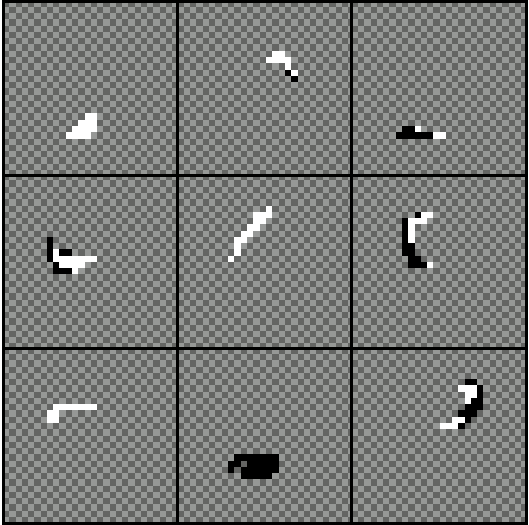
\includegraphics[width=0.18\columnwidth]
    {figures/bmnist-mpe-i} \label{fig:bmnist-mpe-i}\hspace{6pt}
  %\subfloat[]{
    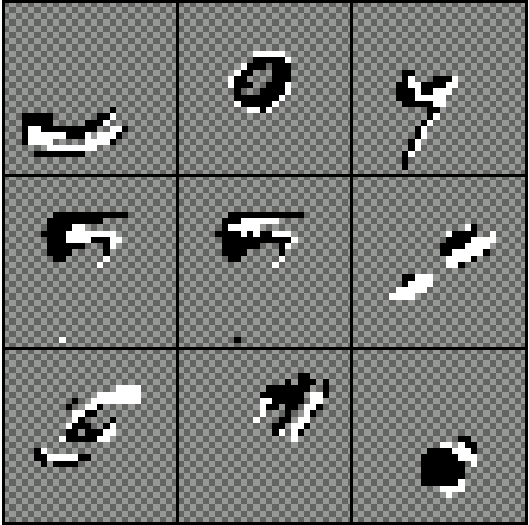
\includegraphics[width=0.18\columnwidth]
    {figures/bmnist-mpe-ii} \label{fig:bmnist-mpe-ii}\hspace{6pt}
  %\subfloat[]{
    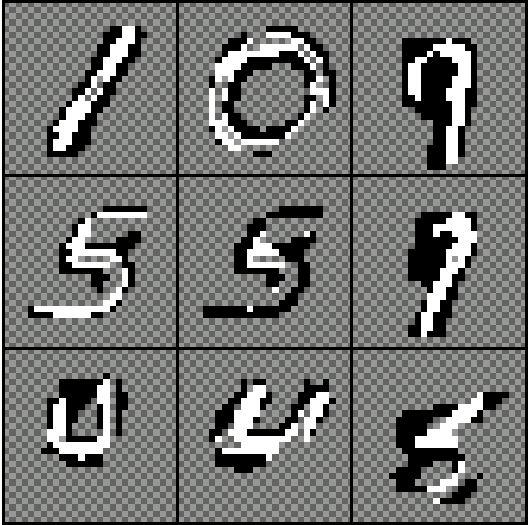
\includegraphics[width=0.18\columnwidth]
    {figures/bmnist-mpe-iii} \label{fig:bmnist-mpe-iii}\hspace{6pt}
  %\subfloat[]{
    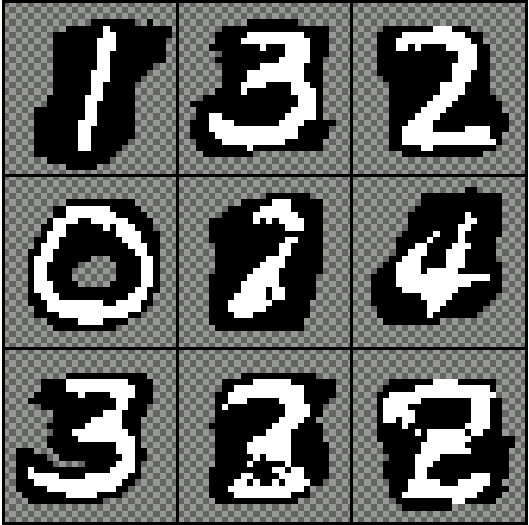
\includegraphics[width=0.18\columnwidth]
    {figures/bmnist-mpe-iiii} \label{fig:bmnist-mpe-iiii}%}

  \end{figure}
E.g., on MNIST, differently complex local patterns emerge
e.g. from small blobs to shape contours and finally full digits\par
\hfill\begin{minipage}{1.0\linewidth}
  \vspace{2pt}
      \raggedleft
      $\color{violet}\boldsymbol\Rightarrow$
a \highlighttext[tomato0]{\emph{\textbf{hierarchy of representations}}}
  structured at levels of abstraction!
\end{minipage}
\end{frame}

\begin{frame}[t]
  \frametitle{\highlighttext[bgrey3]{$\mathsf{CAT}$ vs $\mathsf{ACT}$
    embeddings}}
  \footnotesize
  Even if one can demonstrate that $\mathsf{CAT}$ and $\mathsf{ACT}$
embeddings can lead to the same reconstructions (see
Eq.~\ref{eq:cat-act-eq}), however, \emph{\textbf{they act differently when plugged
in predictive tasks}} (both as feature and target representation spaces).
\begin{minipage}{1.0\linewidth}
 %     \vspace{2pt}
      \raggedleft
      $\color{violet}\boldsymbol\Rightarrow$
      \scriptsize
     \emph{exhaustive empirical evaluation for MLC}
\end{minipage}
\par\bigskip

% While $\mathsf{CAT}$
%  and $\mathsf{ACT}$ embeddings
% for a sample may provide the same decoding
% (see previous Section),
% they may yield very different
% results when exploited for predictive tasks.
%
%
When employed as features for a predictor (its input)
\highlighttext[tomato0]{\emph{\textbf{$\mathsf{ACT}$ embeddings}}} perform better than $\mathsf{CAT}$ ones
due to their \highlighttext[tomato0]{\emph{\textbf{greater information content}}}.
\begin{minipage}{1.0\linewidth}
     \vspace{7pt}
      \raggedleft
      $\color{violet}\boldsymbol\Rightarrow$
      \scriptsize
     \emph{$\mathsf{CAT}$ embeddings are shared more frequently among samples}
\end{minipage}
\par\bigskip
% E.g.~the digits in a cluster in Figure~\ref{fig:bmnist-hid}
% are indistinguishable by their $\mathsf{CAT}$ embeddings while 
% their $\mathsf{ACT}$ representations differ.
% and the additional information of $\mathsf{CAT\text{-}dense}$ to help
% more than placeholders in $\mathsf{CAT\text{-}sparse}$ ones.
%
%

Conversely, when employed to encode target RVs (a predictor's output)
\highlighttext[tomato0]{\textbf{\emph{classification} for the $\mathsf{CAT}$}
\textbf{\emph{case is easier}}} than \emph{regression} with $\mathsf{ACT}$ embeddings.
\begin{minipage}{1.0\linewidth}
    \vspace{7pt}
      \raggedleft
      $\color{violet}\boldsymbol\Rightarrow$
      \scriptsize
     \emph{simpler prediction task due to the sparsity}
\end{minipage}
% since the latter greater variability in values and the 
% simpler prediction task due to the sparsity of the former.
% However, mispredicted $\mathsf{ACT}$ components may still be able to grow a 
% complete tree path, differently from $\mathsf{CAT}$ ones.

 
\end{frame}


\begin{frame}[t]
  \frametitle{\highlighttext[bgrey4]{Partial embedding decoding}}
  \footnotesize

  Up to now we have considered only \textbf{\emph{fully decodable embeddings}},
i.e. embeddings comprising all the information required to materialize a
\textbf{\emph{complete and well-formed 
tree}} necessary to decode $\mathbf{e}$ into $\tilde{\mathbf{x}}$.\par
%obtain 
%the decoded sample 
%
% real case motivation
In some real cases, however, only incomplete
or \highlighttext[tomato0]{\textbf{\emph{partial embeddings}}} are available: some
values $e_{j}$ are corrupted, invalid or just missing.
\begin{minipage}{1.0\linewidth}
 %     \vspace{2pt}
      \raggedleft
      $\color{violet}\boldsymbol\Rightarrow$
      \scriptsize
     \emph{e.g., data compression}
   \end{minipage}\par\bigskip

SPAE routines offer a natural and efficient way to deal with such
cases: MPE inference.
\begin{minipage}{1.0\linewidth}
 %     \vspace{2pt}
      \raggedleft
      $\color{violet}\boldsymbol\Rightarrow$
      \scriptsize
     \emph{treat \highlighttext[tomato0]{\emph{\textbf{missing embedding components as missing values}}}}
   \end{minipage}\par\bigskip


% For the general case, we propose to impute  $\mathsf{CAT}$ and $\mathsf{ACT}$ missing 
% values by performing MPE inference to estimate them.
% For the general case, a principled probabilistic approach is to impute the
% missing embedding values by their MPE values according to $M$.
% %
% Note how this approach generalizes to all nodes in $M$
% what already happens at the leaves
% with $\mathsf{CAT}$ and $\mathsf{ACT}$ decoding.
%
%

In practice, if for an $\mathsf{ACT}$ (resp. $\mathsf{CAT}$) embedding
the component $e_{j}^{i}\notin \mathbf{e}^{i}$ (resp. $z_{j}^{i}\notin \mathbf{z}^{i}$) 
corresponds to a node $n_{j}$ activation (resp. LV $Z_{j}$ state),
then it can be imputed
% $\max_{\mathbf{u}\sim
%   \mathsf{sc}(n_{j})}M_{n_{j}}(\mathbf{u})$
% (resp. $\max_{\mathbf{u}\sim
%   \mathsf{sc}(n_{j})}M_{n_{j}}(\mathbf{u})$)
by employing
$\mathsf{MaxProdMPE}$ on the sub-network $M_{n_{j}}$.
\begin{minipage}{1.0\linewidth}
 %     \vspace{2pt}
      \raggedleft
      $\color{violet}\boldsymbol\Rightarrow$
      \scriptsize
     \emph{imputation for all missing components in one single pass}
   \end{minipage}\par\bigskip

   
\end{frame}


\begin{frame}[t]
    \frametitle{\highlighttext[peas1]{MLC prediction tasks (I)}}
    \footnotesize
    Evaluating SPAE on \emph{\textbf{Multi-Label Classification}}
    (\textbf{MLC}):
predicting the target labels---binary arrays---$\mathbf{y}^{i}\sim \mathbf{Y}$
associated to
sample $\mathbf{x}^{i}\sim\mathbf{X}$.
%as a structured output
%prediction task. 
% MLC is challenging testbed for autoencoders.
\par\bigskip

  Evaluating four \emph{\textbf{different learning scenarios}}:
  \begin{itemize}
  \item no embedding at all (baseline)\par
    \hspace{50pt}{\scriptsize
$\highlight[gold4]{\mathbf{X}\xRightarrow{\scriptscriptstyle p}\mathbf{Y}}$
}
  \item when embedding only input RVs $\mathbf{X}$\par
     \hspace{50pt}{\scriptsize$\highlight[petroil4]{(\mathbf{X}\xrightarrow{\scriptscriptstyle f_{r}}\mathbf{E}_{\mathbf{X}})\xRightarrow{\scriptscriptstyle \mathsf{LR}}\mathbf{Y}}$}
  \item when embedding only target RVs $\mathbf{Y}$ (\emph{requires decoding!})\par
    \hspace{50pt}{\scriptsize$\highlight[purple]{(\mathbf{X}\xRightarrow{\scriptscriptstyle p}(\mathbf{Y}\xrightarrow{\scriptscriptstyle f_{t}}\mathbf{E}_{\mathbf{Y}}))\xrightarrow{\scriptscriptstyle g_{t}}\mathbf{Y}}$}
  \item when embedding both RV sets $\mathbf{X}$, $\mathbf{Y}$\par
     \hspace{50pt}{\scriptsize$\highlight[lacamdarklilac]{((\mathbf{X}\xrightarrow{\scriptscriptstyle f_{r}}\mathbf{E}_{\mathbf{X}})\xRightarrow{\scriptscriptstyle p}(\mathbf{Y}\xrightarrow{\scriptscriptstyle f_{t}}\mathbf{E}_{\mathbf{Y}}))\xrightarrow{\scriptscriptstyle g_{t}}\mathbf{Y}}$}
  \end{itemize}\vspace{7pt}

\end{frame}

  \begin{frame}[t]
    \frametitle{\highlighttext[peas1]{MLC prediction tasks (II)}}
    \footnotesize

    
    \resizebox{0.41\textwidth}{!}{\begin{minipage}{0.48\linewidth}\vspace{5pt}
      \begin{table}[!t]
  \centering
  \tiny
  % \caption[datasets]{Average relative test set (percentage) improvements w.r.t $\mathsf{LR}$ on 10 benchmark  datasets  for  multi-label classification. For each scenario, score, and decoding method, best results are bold. The extra two columns use $\mathsf{kNN}$ decoding, 
  % improved scores w.r.t normal decoding are denoted by $\circ$.}
  \setlength{\tabcolsep}{3pt}  
  % \begin{tabular}{lll|rrr}
  \begin{tabular}{llrrrr}
    %\toprule
    %&&&&\multicolumn{2}{c}{$g_{\mathsf{kNN}}$}\\
    % \textsf{Predictor} & \textsf{Encoder} & \textsf{Decoder}
    % & {$\mathsf{JAC}$} & {$\mathsf{HAM}$} & {$\mathsf{EXA}$} \\
    %&& {$\mathsf{JAC}$} & {$\mathsf{EXA}$}\\% & {$\mathsf{JAC}$} & {$\mathsf{EXA}$} \\
    %\cmidrule{3-4}
    % \midrule
    % \midrule
    %\toprule
    \multirow{3}{*}{\rotatebox[origin=c]{90}{\highlighttext[gold4]{baseline}}}&\multicolumn{1}{l}{${\mathbf{X}\xRightarrow{\scriptscriptstyle p}\mathbf{Y}}$}& {$\mathsf{JAC}$} & {$\mathsf{EXA}$}\\
    %\midrule
    \cmidrule(r){2-4}
    &$p\colon\mathsf{LR}$  & 0.00& 0.00\\
    &$p\colon\mathsf{CRF}_{\mathsf{SSVM}}$ & +15.83& +103.90\\
    \cmidrule[2pt](r){1-4}
    % \multirow{7}{*}{\rotatebox[origin=c]{90}{\highlighttext[petroil4]{scenario I}}}&\multicolumn{3}{l}{${(\mathbf{X}\xrightarrow{\scriptscriptstyle f_{r}}\mathbf{E}_{\mathbf{X}})\xRightarrow{\scriptscriptstyle \mathsf{LR}}\mathbf{Y}}$}\\
    \multirow{6}{*}{\rotatebox[origin=c]{90}{\highlighttext[petroil4]{scenario I}}}\\%&\multicolumn{3}{l}{${(\mathbf{X}\xrightarrow{\scriptscriptstyle f_{r}}\mathbf{E}_{\mathbf{X}})\xRightarrow{\scriptscriptstyle \mathsf{LR}}\mathbf{Y}}$}\\
    %\midrule
    %\cmidrule(r){2-4} 
        &$r\colon\mathsf{RBM}_{h\in\{500,1000,5000\}}$ & +1.46&  -1.62\\
    &$r\colon\mathsf{MADE}_{h\in\{500,1000\}}$ & +2.57&  +2.99\\
    &$r\colon\mathsf{CAE}_{\gamma\in\{0.7,0.8,0.9\}}$ & -0.15&  +4.13\\
    &$r\colon\mathsf{DAE}_{\gamma\in\{0.7,0.8,0.9\}}$ & +0.70&  +4.17\\
    &$r\colon\mathsf{SPAE}_{\mathsf{ACT}}$ & \textbf{+3.54} & \textbf{+17.18} \\%&\multicolumn{2}{c}{$g_{\mathsf{kNN}}$}\\
    &$r\colon\mathsf{SPAE}_{\mathsf{CAT}}$ & -11.90&  -11.53 \\%& {$\mathsf{JAC}$} & {$\mathsf{EXA}$}\\
    %&$r\colon\mathsf{MPN}_{\mathsf{CAT}\text{-}\mathsf{dense}}$ & -4.11& -6.93\\
    %\midrule
    %\cmidrule{2-2} \cmidrule(l){5-6}
     \cmidrule(r){2-4} %\cmidrule(l){5-6}
    % \parbox[t]{2mm}{\multirow{5}{*}{\rotatebox[origin=c]{90}{$\mathbf{X}\rightarrow
    % \mathbf{E}_{\mathbf{Y}}$}}} 
    % &$\mathsf{MADE}_{h=200}$ & 28.05& 85.75& 11.92\\
    % $\mathbf{X}$&$\mathsf{MADE}_{h=200}$ & $\mathsf{RR}$& $\mathsf{MADE}$ & -30.76& +7.10& -29.71\\
    % \multirow{7}{*}{\rotatebox[origin=c]{90}{\highlighttext[purple]{scenario II}}}&\multicolumn{3}{l}{${(\mathbf{X}\xRightarrow{\scriptscriptstyle p}(\mathbf{Y}\xrightarrow{\scriptscriptstyle f_{t}}\mathbf{E}_{\mathbf{Y}}))\xrightarrow{\scriptscriptstyle g_{t}}\mathbf{Y}}$}\\
    \multirow{6}{*}{\rotatebox[origin=c]{90}{\highlighttext[purple]{scenario II}}}\\%&\multicolumn{3}{l}{${(\mathbf{X}\xRightarrow{\scriptscriptstyle p}(\mathbf{Y}\xrightarrow{\scriptscriptstyle f_{t}}\mathbf{E}_{\mathbf{Y}}))\xrightarrow{\scriptscriptstyle g_{t}}\mathbf{Y}}$}\\
    %\midrule
    %\cmidrule{2-2}
    % \cmidrule(r){2-4} %\cmidrule(l){5-6}
    &$t\colon\mathsf{MADE}_{h\in\{200,500\}},p\colon\mathsf{RR}$ & -30.42&  -28.02\\%& $\circ$+14.57&  $\circ$+88.62\\
    &$t\colon\mathsf{SAE}_{\gamma\in\{0.7,0.8,0.9\}},p\colon\mathsf{RR}$
       & +5.96&  +95.78\\%&  - & -\\
    &$t\colon\mathsf{CAE}_{\gamma\in\{0.7,0.8,0.9\}},p\colon\mathsf{RR}$ & +7.60&  +78.81\\%& $\circ$\textbf{+25.81}&  +132.03\\
    &$t\colon\mathsf{DAE}_{\gamma\in\{0.7,0.8,0.9\}},p\colon\mathsf{RR}$ & +13.39&  +102.22\\%& $\circ$+17.01&  +71.20\\
    %&$t\colon\mathsf{SPAE}_{\mathsf{ACT}}$ & +11.65&  +96.30 & \textbf{+27.10}& +133.02\\
    &$t\colon\mathsf{SPAE}_{\mathsf{ACT}},p\colon\mathsf{RR}$ & +15.19&  +98.58\\%& $\circ$+21.94&  $\circ$+107.00\\
    &$t\colon\mathsf{SPAE}_{\mathsf{CAT}},p\colon\mathsf{LR}$ & \textbf{+24.07}&  \textbf{+141.81}\\%& +22.83&  \textbf{+134.43}\\
    %$t\colon\mathsf{MPN}_{\mathsf{CAT}\text{-}\mathsf{dense}},p\colon\mathsf{LR}$ & +19.61&  +119.70& +19.61&  +119.70\\
    %\midrule
    \cmidrule(r){2-4} %\cmidrule(l){5-6}
    % \parbox[t]{2mm}{\multirow{6}{*}{\rotatebox[origin=c]{90}{$\mathbf{E}_{\mathbf{X}}\rightarrow
    % \mathbf{E}_{\mathbf{Y}}$}}}
    % &$\mathsf{MADE}_{h_{\mathbf{X}}=500,h_{\mathbf{Y}}=200}$ & 29.22& 85.71& 12.01\\
    % &$\mathsf{MADE}_{h_{\mathbf{X}}=500,h_{\mathbf{Y}}=500}$ & 29.40& 85.63& 12.00\\
    % &$\mathsf{MADE}_{h_{\mathbf{X}}=1000,h_{\mathbf{Y}}=200}$ & 29.24& 85.64& 11.7\\
    % $\mathsf{MADE}_{h=500}$ &$\mathsf{MADE}_{h=200}$ & $\mathsf{RR}$& $\mathsf{MADE}$ & -28.14& +7.10& -28.00\\
    % $\mathsf{MADE}_{h=500}$ &$\mathsf{MADE}_{h=500}$ & $\mathsf{RR}$& $\mathsf{MADE}$ & -27.81& +6.93& -27.14\\
    % $\mathsf{MADE}_{h=1000}$ &$\mathsf{MADE}_{h=200}$ & $\mathsf{RR}$& $\mathsf{MADE}$ & -27.80& +6.96& -29.03\\
    % \multirow{7}{*}{\rotatebox[origin=c]{90}{\highlighttext[lacamdarklilac]{scenario III}}}&\multicolumn{3}{l}{${((\mathbf{X}\xrightarrow{\scriptscriptstyle f_{r}}\mathbf{E}_{\mathbf{X}})\xRightarrow{\scriptscriptstyle p}(\mathbf{Y}\xrightarrow{\scriptscriptstyle f_{t}}\mathbf{E}_{\mathbf{Y}}))\xrightarrow{\scriptscriptstyle g_{t}}\mathbf{Y}}$}\\
    \multirow{6}{*}{\rotatebox[origin=c]{90}{\highlighttext[lacamdarklilac]{scenario III}}}\\%&\multicolumn{3}{l}{${((\mathbf{X}\xrightarrow{\scriptscriptstyle f_{r}}\mathbf{E}_{\mathbf{X}})\xRightarrow{\scriptscriptstyle p}(\mathbf{Y}\xrightarrow{\scriptscriptstyle f_{t}}\mathbf{E}_{\mathbf{Y}}))\xrightarrow{\scriptscriptstyle g_{t}}\mathbf{Y}}$}\\
    %\midrule
    %\cmidrule{2-2}
    % \cmidrule(r){2-4} %\cmidrule(l){5-6}
    &$r, t\colon\mathsf{MADE},p\colon\mathsf{RR}$ & -27.15&  -25.14\\%& +12.77&  +85.78\\
    &$r, t\colon\mathsf{CAE}_{\gamma\in\{0.7,0.8,0.9\}},p\colon\mathsf{RR}$ & +5.21&  +79.20\\%& $\circ$+24.32&  $\circ$+125.21\\
    &$r, t\colon\mathsf{DAE}_{\gamma\in\{0.7,0.8,0.9\}},p\colon\mathsf{RR}$ & +13.97&  +98.25\\%& $\circ$+16.67&  +76.17\\
    %$r\colon\mathsf{SPAE}_{\mathsf{ACT}},t\colon\mathsf{MPN}_{\mathsf{ACT}\text{-}\mathsf{full}},p\colon\mathsf{RR}$ & +14.52&  +106.62&\textbf{+25.41}&  +129.60\\
    &$r\colon\mathsf{SPAE}_{\mathsf{ACT}},t\colon\mathsf{SPAE}_{\mathsf{ACT}},p\colon\mathsf{RR}$ &+15.98&  +106.65\\%&$\circ$+21.45&  $\circ$+109.7\\
    &$r\colon\mathsf{SPAE}_{\mathsf{CAT}},t\colon\mathsf{SPAE}_{\mathsf{CAT}},p\colon\mathsf{LR}$ &+13.73&  +107.05\\%&+11.61& +102.08\\
    %$r\colon\mathsf{SPAE}_{\mathsf{CAT}\text{-}\mathsf{dense}},t\colon\mathsf{MPN}_{\mathsf{CAT}\text{-}\mathsf{dense}},p\colon\mathsf{LR}$ %&+17.81&  +111.24&+14.20&  +68.38\\
    &$r\colon\mathsf{SPAE}_{\mathsf{ACT}},t\colon\mathsf{SPAE}_{\mathsf{CAT}},p\colon\mathsf{LR}$ & \textbf{+25.47} &  \textbf{+144.78}\\%& \textbf{+23.47} & \textbf{+135.36}\\
     \cmidrule(r){2-4} %\cmidrule(l){5-6}

   % \bottomrule
  \end{tabular}
  \label{tab:aggr-scores}
\end{table}

\end{minipage}}\hspace{30pt}
\begin{minipage}{0.47\linewidth}
  \vspace{0pt}
  \raggedright
  \scriptsize
% Applying
%   SPAE for MLC predictions.\par\vspace{10pt}

%   Evaluating three different scenarios:
%   \begin{itemize}
%   \item when embedding only input RVs\par
%     \hfill {\scriptsize$\highlight[petroil4]{(\mathbf{X}\xrightarrow{\scriptscriptstyle f_{r}}\mathbf{E}_{\mathbf{X}})\xRightarrow{\scriptscriptstyle \mathsf{LR}}\mathbf{Y}}$}
%   \item when embedding only target RVs\par
%     \hfill {\scriptsize$\highlight[purple]{(\mathbf{X}\xRightarrow{\scriptscriptstyle p}(\mathbf{Y}\xrightarrow{\scriptscriptstyle f_{t}}\mathbf{E}_{\mathbf{Y}}))\xrightarrow{\scriptscriptstyle g_{t}}\mathbf{Y}}$}
%   \item when embedding both
%      {\scriptsize$\highlight[lacamdarklilac]{((\mathbf{X}\xrightarrow{\scriptscriptstyle f_{r}}\mathbf{E}_{\mathbf{X}})\xRightarrow{\scriptscriptstyle p}(\mathbf{Y}\xrightarrow{\scriptscriptstyle f_{t}}\mathbf{E}_{\mathbf{Y}}))\xrightarrow{\scriptscriptstyle g_{t}}\mathbf{Y}}$}
%    \end{itemize}\vspace{7pt}

  Measuring the average relative improvement for for the \textsf{JAC}card,
  \textsf{HAM}ming and \textsf{EXA}ct match scores
  over \emph{\textbf{10 standard MLC benchmark datasets}}.\par\bigskip
  
  In all scenarios we employ a \textbf{linear predictor}: a logistic
  (\textsf{LR}) or ridge regressor (\textsf{RR}) for classification or
  regression, respectively.\par\bigskip
  
  Both $\mathsf{ACT}$ and $\mathsf{CAT}$ are competitive, in all
  scenarios---for all scores---against:
  \begin{itemize}
  \item $\mathsf{RBMs}$
  \item probabilistic autoencoders ($\mathsf{MADEs}$)
  \item deep stacked autoencoders ($\mathsf{SAEs}$)
  \item contractive autoencoders ($\mathsf{CAEs}$)
    \item denoising autoencoders ($\mathsf{DAEs}$)
  \end{itemize}


\end{minipage}
  \end{frame}



    \begin{frame}[t]
  \frametitle{\highlighttext[peas1]{Why SPAE works for RL\dots}}
  \footnotesize
  \begin{minipage}[t]{0.3\linewidth}
      %\begin{center}
         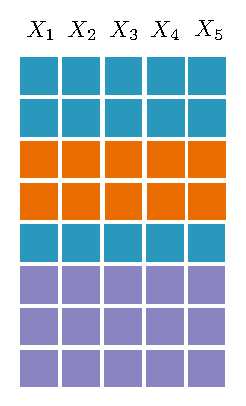
\includegraphics[width=0.5791\linewidth]{figures/grid-1}
      %\end{center}
    \end{minipage} \hspace{10pt}\begin{minipage}[t]{0.3\linewidth}
      %\begin{center}
        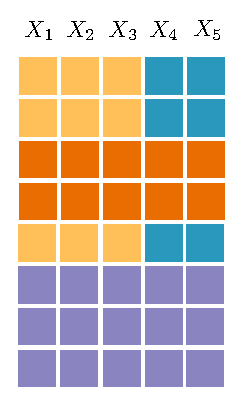
\includegraphics[width=0.5832\linewidth]{figures/grid-2}
      %\end{center}
    \end{minipage}
    \hspace{10pt}\begin{minipage}[t]{0.3\linewidth}
      %\begin{center}
        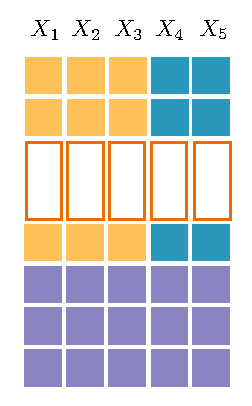
\includegraphics[width=0.59535\linewidth]{figures/grid-3}
      %\end{center}
    \end{minipage}
  \vspace{5pt}
  \raisebox{0pt}{\begin{minipage}[t]{0.3\linewidth}
        %\begin{center}
          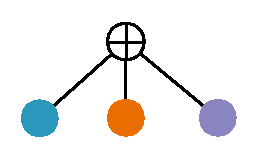
\includegraphics[width=0.5791\linewidth]{figures/learnspn-1}
        %\end{center}
      \end{minipage}}\hspace{4pt}\raisebox{-20pt}{\begin{minipage}[t]{0.3\linewidth}
        %\begin{center}
          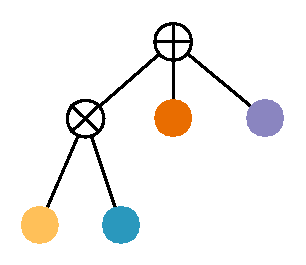
\includegraphics[width=0.6723\linewidth]{figures/learnspn-2}
        %\end{center}
      \end{minipage}}\hspace{1pt}\raisebox{-18pt}{\begin{minipage}[t]{0.3\linewidth}
        %\begin{center}
          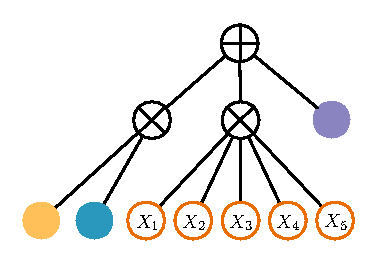
\includegraphics[width=0.81\linewidth]{figures/learnspn-3}
        %\end{center}
      \end{minipage}}\par\bigskip
  SPNs are built via \emph{hierarchical co-clustering}, learning
  features as \textbf{\emph{recursive data
      crawlers}}!\customcitenomark{Vergari2015}\customcitenomark{Gens2013}
\end{frame}

\begin{frame}[t]
  \frametitle{\highlighttext[peas1]{Partial embedding decoding}}
  \footnotesize
   Evaluating the \emph{\textbf{resilience to missing-at-random}} embedding components
when decoding $\mathsf{CAT}$ and $\mathsf{ACT}$ label embeddings in scenario II---varying from 0 (full
embedding) to 90\% missing, by increments of 10\
% We compare our two imputation schemes: either employing $\mathsf{MaxProdMPE}$ to
% estimate the most probable component (-$\mathsf{mpe}$) or re-evaluating the MPN bottom-up
% to compute the missing predicted activations (denoted as $\mathsf{ACT}\text{-}\mathsf{reev}$).
%
  \begin{figure}
   \raggedright
     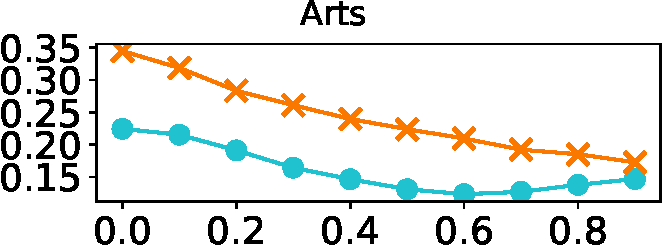
\includegraphics[width=0.22\columnwidth]
     {figures/Arts-EXACT-cat-crop.pdf}\hspace{2pt}
     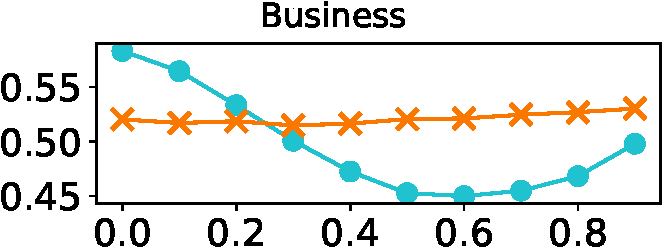
\includegraphics[width=0.22\columnwidth]
     {figures/Business-EXACT-cat-crop.pdf}\hspace{2pt}
     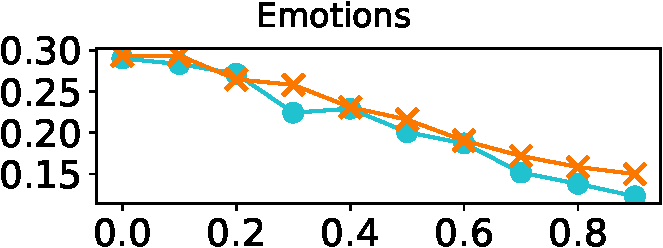
\includegraphics[width=0.22\columnwidth]
     {figures/Emotions-EXACT-cat-crop.pdf}\\[2pt]
     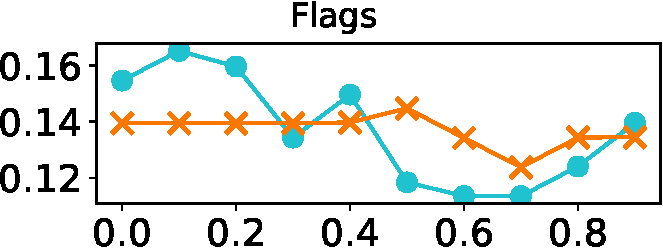
\includegraphics[width=0.22\columnwidth]
     {figures/Flags-EXACT-cat-crop.pdf}\hspace{2pt}
     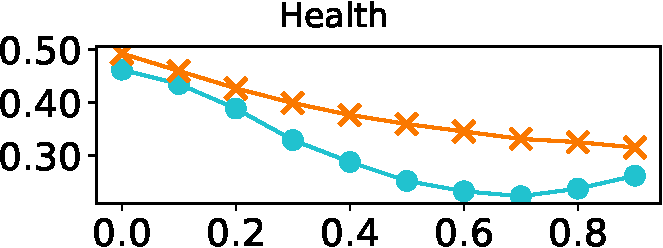
\includegraphics[width=0.22\columnwidth]
     {figures/Health-EXACT-cat-crop.pdf}\hspace{2pt}
     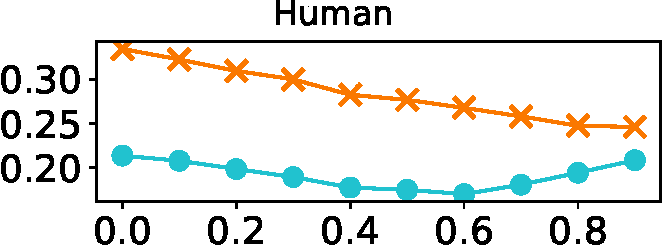
\includegraphics[width=0.22\columnwidth]
     {figures/Human-EXACT-cat-crop.pdf}\\[2pt]
     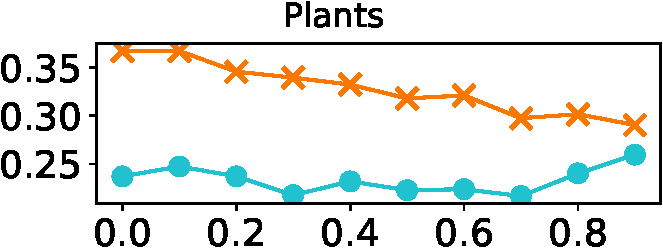
\includegraphics[width=0.22\columnwidth]
     {figures/Plants-EXACT-cat-crop.pdf}\hspace{2pt}
     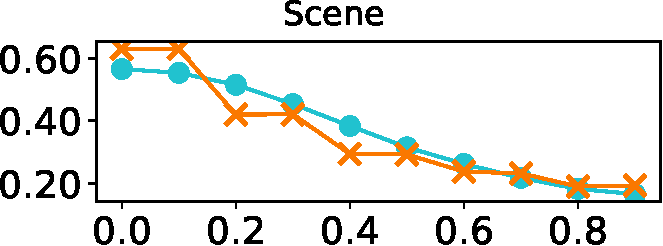
\includegraphics[width=0.22\columnwidth]
     {figures/Scene-EXACT-cat-crop.pdf}\hspace{2pt}
     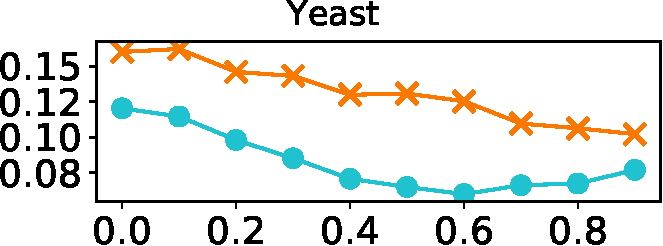
\includegraphics[width=0.22\columnwidth]
     {figures/Yeast-EXACT-cat-crop.pdf}%\\[15pt]
   \label{fig:miss-exa}
 \end{figure}




% Either we apply the MPE inference imputation scheme on these
% missing components or we evaluate the MPN bottom-up, computing the
% missing predicted activation by evaluating the children ones according
% to the corresponding node type.
% If leaves activations are missing, their MPE activation is
% considered.
% After a full embedding is comleted by imputation, the decoding phase
% proceeds as before.
%
%
% Figure~\ref{fig:miss-exa} summarizes the  $\mathsf{EXA}$ results for $\mathsf{CAT}$ and $\mathsf{ACT}$ decoding
% % $\mathsf{ACT}\text{-}\mathsf{mpe}$, $\mathsf{ACT}\text{-}\mathsf{reev}$ and $\mathsf{CAT}\text{-}\mathsf{mpe}$ %,  perform
% %differently for the $\mathsf{EXA}$ score 
% on 9 datasets (the $\mathsf{EXA}$ score on Cal is always 0).
Both $\mathsf{CAT}$ and $\mathsf{ACT}$ decoding routines are quite
robust
\begin{minipage}{1.0\linewidth}
 %     \vspace{2pt}
      \raggedleft
      $\color{violet}\boldsymbol\Rightarrow$
      \scriptsize
     \emph{degrading performances by less than $50\%$ with $50\%$ missing components}
\end{minipage}\par\bigskip
$\mathsf{CAT}$ scores decay slower than $\mathsf{ACT}$ and are generally better
\end{frame}


\begin{frame}[t]
  \frametitle{\highlighttext[peas1]{Conclusions}}
  \footnotesize
  We extend the scope of SPNs towards Representation
Learning (RL). \par
% We leverage their learned inner representations so as 
% to disentangle and uncover different explanatory
% factors behind the data
% in order to use them later for predictive tasks.
%such that they could later be exploited in several other tasks or domains, often 
%boosting performance. 
%In a common RL scenario,
%The feature representations are often 
%Typically, this is done by extracted by a model learned in an unsupervised
%fashion and typically lead to improved performance when predicting previously
%unseen target labels.
%
% Why is this interesting? What has already been done?
% Half related works/half motivational part
% Unsupervisedly trained generative models have been largely
% employed as feature extractors.
Compared to other classical probabilstic models (\textsf{RBMs},
\textsf{MADEs}) and autoencoders (\textsf{CAEs}, \textsf{DAEs},
\textsf{SAE}, etc.) for
RL, SPNs in our SPAE routines can:
\begin{itemize}
\item still be used as tractable models for exact inference on a \emph{\textbf{wider
  range of queries}}
\item provide \textbf{\emph{rich}, \emph{hierarchical} and \emph{part-based}
  features}
  \item save \emph{time and effort} in hyperparameter tuning
since both their structure and weights can be learned
 in a ``cheap'' way---e.g., adaptive size
\end{itemize}\bigskip

SPAE  suggests  several  interesting  avenues for future work:
%dependencies among the latent variables, 
\begin{itemize}
\item explore embeddings
  based on other instances of Arithmetic Circuits~\parencite{Darwiche2009}
\item extracting \emph{\textbf{structured
  representations}}
  \item perform \emph{\textbf{differentiable MPE inference}} allowing SPNs---bridging the gap even more between SPNs, autoencoders
and other neural networks.
\end{itemize}
\end{frame}


\begin{frame}[t]
  \frametitle{\highlighttext[yellow3]{Shameless plug}}
  \footnotesize
  {\Large\highlighttext[lacamlilac]{I} } Star or fork the \emph{\textbf{awesome-spn}} repo for more references to the SPN literature:\vspace{-5pt}
  \begin{center}
    \large\url{https://github.com/arranger1044/awesome-spn}
  \end{center}\par\bigskip


  {\Large\highlighttext[lacamlilac]{II} }Visit our poster for more on SPN structure learning tomorrow, \emph{Main
  Track Session 1}\vspace{-5pt}
  \begin{center}
    \large{\emph{\textbf{``Alternative Variable Splitting Methods to Learn Sum-Product Networks''}}}
  \end{center}\vspace{-5pt}

   joint work with Nicola Di Mauro, Floriana Esposito and Fabrizio Ventola \par\bigskip\bigskip
  
  {\Large\highlighttext[lacamlilac]{III} }\emph{\textbf{Are you looking for a post-doc}} to work on \emph{probabilistic models}, \emph{deep
    learning} and \emph{machine learning}?
  Here is my cv:\vspace{-5pt}
  \begin{center}
    %\vspace{-10pt}
    \large\url{tinyurl.com/ycnhn7nu}
  \end{center}
\end{frame}
 
\begin{frame}[allowframebreaks]
  \frametitle{References}
  \setlength\bibitemsep{8pt}
  \printbibliography
\end{frame}

\begin{frame}
  \frametitle{Discuss}
\footnotesize
\begin{table}
  \setlength{\tabcolsep}{10pt}
    \centering
    \begin{tabular}{cccc}
      \raisebox{-3pt}{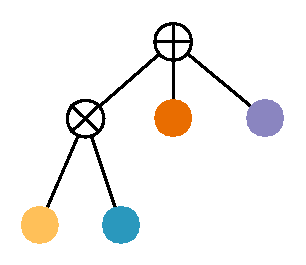
\includegraphics[width=0.2\linewidth]{figures/learnspn-2}}&\raisebox{-4pt}{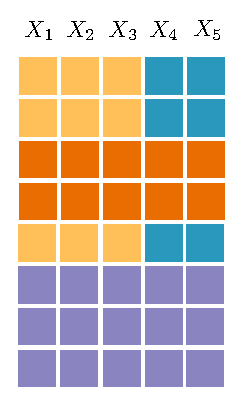
\includegraphics[width=0.15\linewidth]{figures/grid-2}}&   %  $
%                                                                                                                         \begin{aligned}
%                                                                                                                              \mathbf{S}^{\oplus}(\mathbf{x}) &=
%                                      {\color{gold6}\log}({\color{petroil4}\mathbf{W}}\mathbf{x})\\                                                                       \mathbf{S}^{\otimes}(\mathbf{x}) &= {\color{gold6}\exp}({\color{petroil4}\mathbf{P}}\mathbf{x})                                         
%                                                                                                                         \end{aligned}
%                                                                                                                         $
                                                                                                                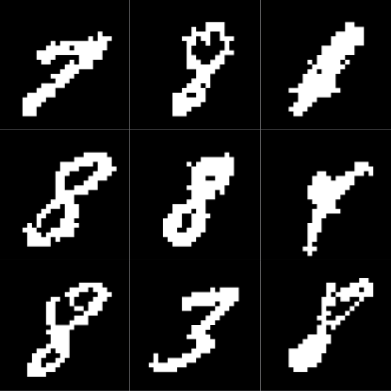
\includegraphics[width=0.2\columnwidth]
    {figures/hid-clu-4}                                                                                              
&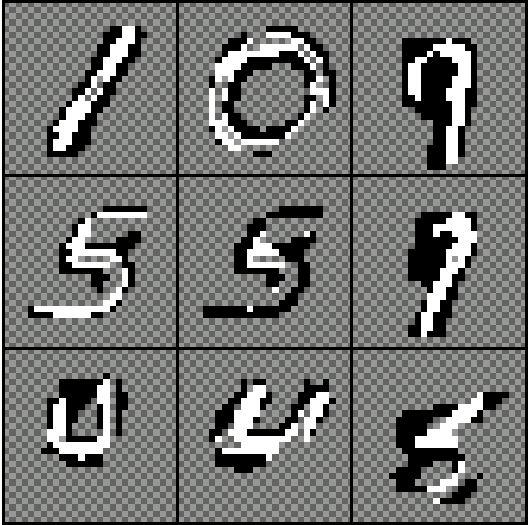
\includegraphics[width=0.2\columnwidth]
    {figures/bmnist-mpe-iii}\\
    %   \includegraphics[width=0.25\columnwidth]{figures/australian-2-crop-7}&
    %                                                                          \includegraphics[width=0.2\columnwidth]{figures/cond-samples-16}&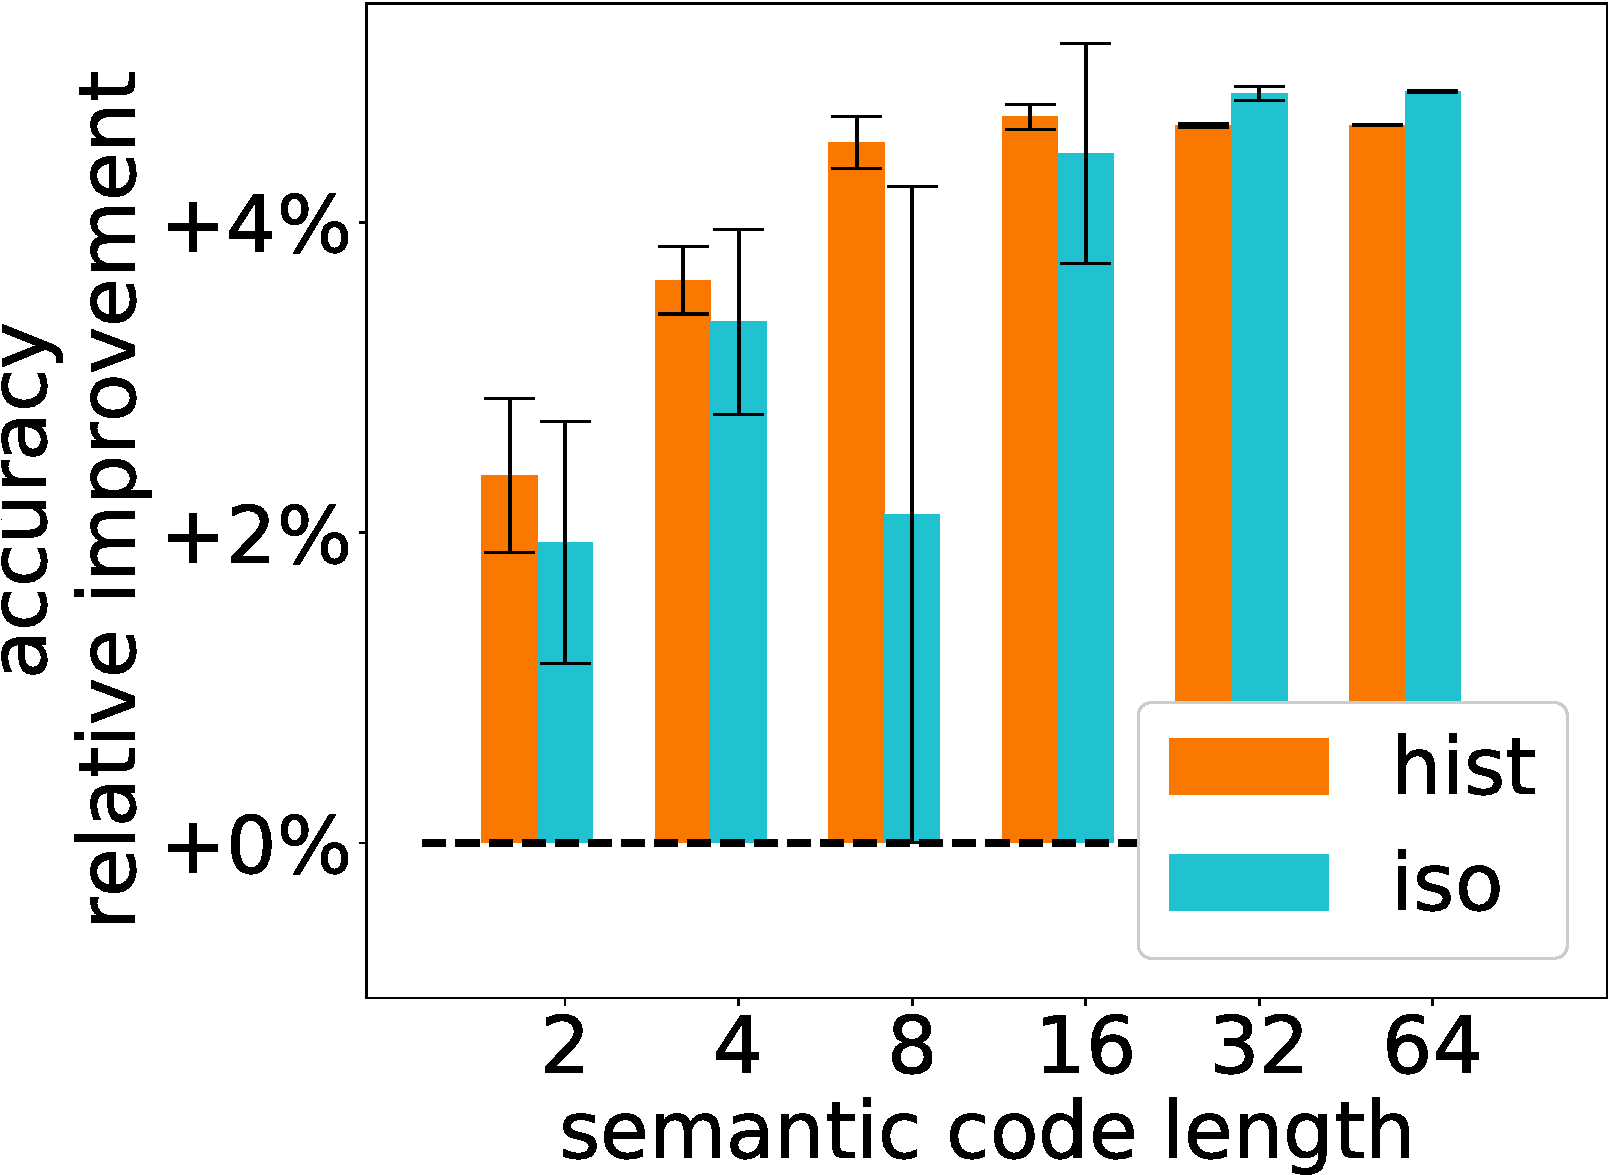
\includegraphics[width=0.25\columnwidth]{figures/test-mpe-acc-crop}&
    %   % \includegraphics[width=0.07\columnwidth]{figures/orig-16-crop}
    % \includegraphics[width=0.05\columnwidth]{figures/dec-left-16-crop}
    % \includegraphics[width=0.05\columnwidth]{figures/dec-right-16-crop}
    % \includegraphics[width=0.05\columnwidth]{figures/dec-up-16-crop}
    % \includegraphics[width=0.05\columnwidth]{figures/dec-down-16-crop}\\
    \end{tabular}
  \end{table}
\end{frame}



\end{document}

%%% Local Variables:
%%% mode: latex
%%% TeX-engine: xetex
%%% TeX-master: t
%%% End:

